% !TeX root = RJwrapper.tex
\title{datadriftR: An R Package for Concept Drift Detection in Predictive Models}


\author{by Ugur Dar and Mustafa Cavus}

\maketitle

\abstract{%
Predictive models often degrade due to data drift, particularly concept drift, where the relationship between variables and the response changes. Traditional detection methods based on accuracy or variable distributions often miss subtle concept drifts. This paper presents, an R package for detecting concept drift and introduces a novel method, Profile Drift Detection (PDD). PDD leverages explainable artificial intelligence tool Partial Dependence Profiles (PDPs) to detect and explain drift causes. It quantifies PDP changes using innovative metrics, balancing sensitivity and computational efficiency. Aligned with MLOps practices, this approach focuses on model monitoring and adaptive retraining in dynamic environments. Experiments on synthetic and real-world datasets show that PDD outperforms existing methods, maintaining high accuracy while ensuring stability. The results demonstrate its robustness for real-time applications and ability to adapt models effectively. The paper discusses its advantages, limitations and potential extensions for broader applications.
}

\hypertarget{introduction}{%
\section{Introduction}\label{introduction}}

Predictive models assume train and test data are independent and identically distributed \citep{cieslak_and_chawla_2009} but this rarely holds, reducing performance \citep{alaiz_et_al_2008}. As data evolves, models must adapt \citep{moreno_et_al_2012} while ensuring accuracy and efficiency \citep{korycki_and_krawczyk_2023}. Model monitoring, a key MLOps component, maintains ML consistency in real-world applications (Figure\textasciitilde{}\ref{fig:mdp}) \citep{biecek_2019, mougan_and_nielsen_2023}.

\begin{figure}[H]

{\centering 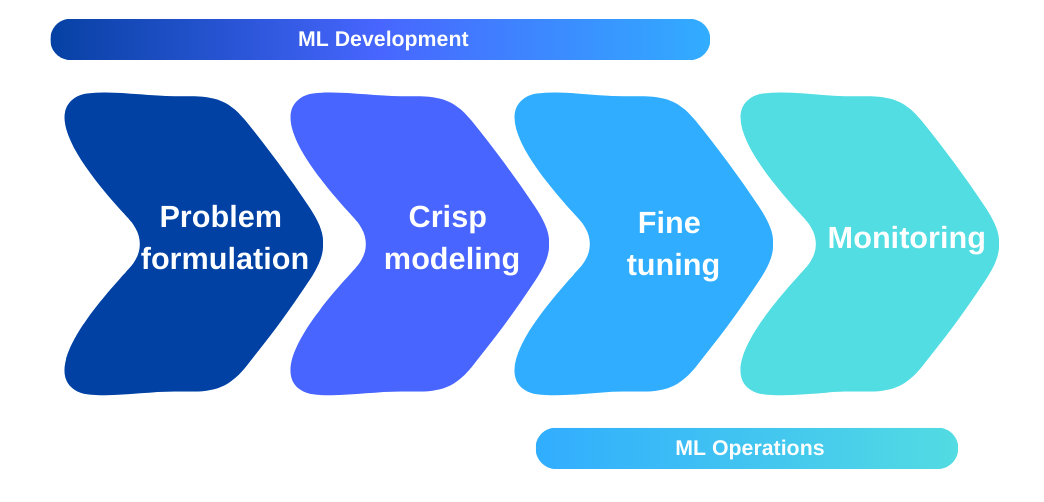
\includegraphics[width=0.8\linewidth,height=0.2\textheight]{figures/mdp_resize} 

}

\caption{The predictive modeling process}\label{fig:mdp}
\end{figure}

Data drift, classified into covariate, label and concept drift, disrupts model behavior. It appears in scenarios like pandemic-driven electricity demand \citep{fumagalli_et_al_2023}, airline customer shifts \citep{garg_et_al_2021} and supply chain changes \citep{kulinski_and_inouye_2023}. Timely detection is crucial for model reliability.

Data drift detection methods fall into statistical, sequential and window-based categories. Concept drift, a change in explanatory-response variable relationships, often eludes traditional methods \citep{demvsar_and_bosnic_2018, duckworth_et_al_2021, rahmani_et_al_2023}. This underscores the need for MLOps, which integrates model monitoring and adaptation to maintain performance in dynamic environments. A key challenge arises when concept drift occurs without shifts in performance or distribution metrics, making conventional detection unreliable and necessitating alternative approaches.

\cite{demvsar_and_bosnic_2018} highlighted that existing drift detection methods rely on performance and distribution metrics, which fail to explain underlying model changes. They proposed a method using local interpretable model-agnostic explanations \citep{strumbelj_et_al_2009}, showing improved detection. \cite{duckworth_et_al_2021} used normalized SHAP \citep{lundberg_2017} to detect drift in emergency department models post-COVID-19.

\cite{muschalik_et_al_2022} developed a concept drift detection approach using permutation-based variable importance \citep{breiman2001random}, emphasizing the need for improvements in complexity, sensitivity and explainability. \cite{rahmani_et_al_2023} found SHAP effective for variable importance but insufficient for distinguishing covariate and concept drift. \cite{mougan_and_nielsen_2023} warned that statistical tests rely on data distribution alone, causing false alarms and proposed an explainable method using bootstrap uncertainty estimation and SHAP.

\cite{mattos_et_al_2021} addressed the lack of explainability in concept drift detection by developing a decision tree-based technique but noted its limitations, including high training costs and difficulty tracking variables in non-tree models. \cite{fumagalli_et_al_2023} extended permutation-based variable importance for incremental models but stressed the need to improve efficiency, complexity and sensitivity.

XAI-based data drift detection methods are limited and often rely on high-cost approaches like permutation-based importance or SHAP, which are not always practical for detecting changes in response-explanatory variable relationships. To address this, we propose a solution using Partial Dependence Profiles (PDP), a versatile XAI tool for examining response-explanatory relationships, hyper-parameter optimization \citep{moosbauer_et_al_2021} and variable importance analysis \citep{inglis_et_al_2022}.

Software implementing complex drift detection methods is also scarce. R tools like \CRANpkg{vetiver} and \CRANpkg{pins} monitor model metrics but lack dedicated drift detection. \CRANpkg{drifter} detects drift via distribution distances and PDPs but is limited to comparing trained models, while \CRANpkg{harbinger} focuses on time series anomalies. In contrast, Python offers advanced tools such as EvidentlyAI\footnote{\href{https://www.evidentlyai.com/}{https://www.evidentlyai.com/}}, SeldonIO\footnote{\href{https://www.seldon.io/}{https://www.seldon.io/}}, NannyML\footnote{\href{https://nannyml.readthedocs.io/en/stable/index.html}{https://nannyml.readthedocs.io/en/stable/index.html}}, Frouros\footnote{\href{https://frouros.readthedocs.io/en/latest/}{https://frouros.readthedocs.io/en/latest/}} and River\footnote{\href{https://riverml.xyz/0.8.0/examples/concept-drift-detection/}{https://riverml.xyz/0.8.0/examples/concept-drift-detection/}}.

To bridge these gaps, we introduce \CRANpkg{datadriftR}, an XAI-based concept drift detection package leveraging PDP for real-time monitoring. Our study demonstrates its efficiency in detecting concept drift while providing explanations for model changes. To our knowledge, \CRANpkg{datadriftR} is the first package combining explainable and widely used drift detection methods.

The rest of the paper is structured as follows: the next section discusses data drifts, followed by the concept drift detection methods in the package. We then compare their performance on synthetic and real-world datasets, concluding with future research directions.

\hypertarget{preliminaries}{%
\section{Preliminaries}\label{preliminaries}}

Let \(f_{\theta}: \mathcal{X} \rightarrow \mathcal{Y}\) be a predictive model with parameters \(\theta\), trained on \(D = \{(x_i, y_i)\}_{i=1}^{n}\) to minimize loss \(L(f_{\theta}(x_i), y_i)\). The optimal parameters \(\hat{\theta}\) are found by solving \(\hat{\theta} = \arg \min_{\theta} \sum_{i=1}^{n} L(f_{\theta}(x_i), y_i)\). Data drift occurs when the training distribution \(P_{\text{train}}(X, Y)\) differs from the test distribution \(P_{\text{test}}(X, Y)\), impacting model performance.

\noindent \textbf{Covariate drift.} The explanatory variable distribution changes while the response variable remains the same: \(P_{\text{train}}(X) \neq P_{\text{test}}(X)\), causing prediction difficulties despite good training performance.

\noindent \textbf{Label drift.} The response variable distribution changes while the explanatory variable remains constant: \(P_{\text{train}}(Y) \neq P_{\text{test}}(Y)\), leading to increased misclassification, especially in imbalanced datasets.

\noindent \textbf{Concept drift.} Both explanatory and response variable distributions change: \(P_{\text{train}}(X, Y) \neq P_{\text{test}}(X, Y)\), reducing model accuracy and reliability.

\noindent The next section describes methods for detecting these drifts.

\hypertarget{methods}{%
\section{Methods}\label{methods}}

This section describes the existing drift detection methods such as Drift Detection Method, Early Drift Detection Method, Hoeffding Drift Detection Methods, Kolmogorov-Smirnov test-based Windowing and Page-Hinkley, as well as our proposed concept drift detection method Profile Drift Detection.

\hypertarget{hoeffdings-drift-detection-method-on-average}{%
\subsection{Hoeffding's Drift Detection Method on Average}\label{hoeffdings-drift-detection-method-on-average}}

HDDM-A detects abrupt concept drifts in data streams based on Hoeffding's Inequality. It monitors a simple moving average and evaluates changes using confidence levels \(\alpha_D\) (for drift detection) and \(\alpha_W\) (for alerts).

The data stream is divided into two windows: \textbf{minimum} \((n_{\text{min}}, c_{\text{min}})\) and \textbf{maximum} \((n_{\text{max}}, c_{\text{max}})\), which track past and current states, updating when necessary.

Error bounds for drift detection are computed as:
\begin{equation}
\epsilon_{\alpha_D} = \sqrt{\frac{1}{2n} \ln \left(\frac{1}{\alpha_D}\right)}, \quad
\epsilon_{\alpha_{D1}} = \sqrt{\frac{1}{2n_{\text{min}}} \ln \left(\frac{1}{\alpha_D}\right)}, \quad
\epsilon_{\alpha_{D2}} = \sqrt{\frac{1}{2n_{\text{max}}} \ln \left(\frac{1}{\alpha_D}\right)}
\end{equation}

Windows update if:
\begin{equation}
\frac{c_{\text{min}}}{n_{\text{min}}} + \epsilon_{\alpha_{D1}} \geq \frac{c}{n} + \epsilon_{\alpha_D} \quad \Rightarrow \quad (c_{\text{min}}, n_{\text{min}}) \leftarrow (c, n)
\end{equation}
\begin{equation}
\frac{c_{\text{max}}}{n_{\text{max}}} - \epsilon_{\alpha_{D2}} \leq \frac{c}{n} - \epsilon_{\alpha_D} \quad \Rightarrow \quad (c_{\text{max}}, n_{\text{max}}) \leftarrow (c, n)
\end{equation}

Drift is detected when:
\begin{equation}
\left| \frac{c}{n} - \frac{c_i}{n_i} \right| \geq \sqrt{\frac{n - n_i}{n_i} \frac{1}{2n} \ln \left(\frac{1}{\alpha}\right)}, \quad i \in \{\text{min}, \text{max}\}
\end{equation}

Using \(\alpha = \alpha_D\) detects drift, while \(\alpha = \alpha_W\) triggers an alert state.

\hypertarget{hoeffdings-drift-detection-method-on-weighted}{%
\subsection{Hoeffding's Drift Detection Method on Weighted}\label{hoeffdings-drift-detection-method-on-weighted}}

HDDM-W detects concept drifts in data streams using Exponentially Weighted Moving Averages (EWMA) and Hoeffding's Inequality. The EWMA statistic is computed as:
\begin{equation}
\hat{\mu}_{\text{EWMA}} = \lambda x_i + (1 - \lambda) \hat{\mu}_{\text{EWMA}}
\end{equation}
where \(\lambda \in [0,1]\) controls the weight of recent observations.

HDDM-W is better suited for detecting gradual drifts, while HDDM-A excels at detecting abrupt drifts. Like DDM and EDDM, implementations in \texttt{scikit-multiflow} and \texttt{river} detect drift based on prediction errors, without assuming any specific data distribution.

\hypertarget{kolmogorov-smirnov-windowing-method}{%
\subsection{Kolmogorov-Smirnov Windowing Method}\label{kolmogorov-smirnov-windowing-method}}

KSWIN is a non-parametric drift detection method based on the Kolmogorov-Smirnov (KS) test \citep{raab_2020}. It maintains a sliding window \(\Psi\) of \(n\) observations, splitting it into:

\begin{itemize}
    \item $R$: the most recent $r$ observations,
    \item $W$: $r$ randomly selected older observations.
\end{itemize}

The KS test computes the maximum absolute difference between empirical distributions:
\begin{equation}
dist_{w,r} = \sup_x \left| F_W(x) - F_R(x) \right|
\end{equation}

Drift is detected if:
\begin{equation}
dist_{w,r} > \sqrt{-\frac{\ln \alpha}{r}}
\end{equation}

KSWIN detects drift without distributional assumptions and applies to both response and explanatory variables, identifying changes even before response values are observed.

\hypertarget{page-hinkley-test}{%
\subsection{Page-Hinkley Test}\label{page-hinkley-test}}

The Page-Hinkley Test (PH) detects mean shifts in data streams, similar to Cumulative Sums \citep{sebastiano_fernandes_2017}. It incorporates a forgetting factor \(\alpha\) to reduce the impact of older data. Initially, \(n = 1\), \(x_{\text{ort}} = 0\) and \(S = 0\). For each new observation:

\begin{equation}
x_t = x_{\text{ort}} + \frac{x_t - x_{t-1}}{n}
\end{equation}

\begin{equation}
S_t = \max \left(0, \alpha \cdot S_{t-1} + x_t - x - \delta \right)
\end{equation}

If \(S_t > \lambda\), a concept drift is detected.

PH can be applied to explanatory or response variables and does not require waiting for the response variable's actual value. Unlike KSWIN, PH does not include an alert state.

\hypertarget{drift-detection-method-ddm}{%
\subsection{Drift Detection Method (DDM)}\label{drift-detection-method-ddm}}

DDM estimates error rate variability using:
\begin{equation}
s_i = \sqrt{\frac{p_i(1 - p_i)}{i}}
\end{equation}
For large samples, the error rate follows a normal distribution with a confidence interval:
\begin{equation}
p_i \pm \alpha \cdot s_i
\end{equation}

Warning Level:
\begin{equation}
p_i + s_i \geq p_{\text{min}} + 2 \cdot s_{\text{min}}
\end{equation}

Drift Level:
\begin{equation}
p_i + s_i \geq p_{\text{min}} + 3 \cdot s_{\text{min}}
\end{equation}
DDM is model-independent and efficient but does not detect virtual drift in explanatory variables.

\hypertarget{early-drift-detection-method-eddm}{%
\subsection{Early Drift Detection Method (EDDM)}\label{early-drift-detection-method-eddm}}

EDDM extends DDM by tracking error distances \citep{baena_garcia_2006}. It computes:
\begin{equation}
p'_i + 2 \cdot s'_i
\end{equation}
and updates \((p'_{\text{max}}, s'_{\text{max}})\) accordingly.

Warning Level:
\begin{equation}
\frac{p'_i + 2 \cdot s'_i}{p'_{\text{max}} + 2 \cdot s'_{\text{max}}} < 0.95
\end{equation}

Drift Level:
\begin{equation}
\frac{p'_i + 2 \cdot s'_i}{p'_{\text{max}} + 2 \cdot s'_{\text{max}}} < 0.90
\end{equation}
When drift occurs, the model is retrained and \((p'_{\text{max}}, s'_{\text{max}})\) are reset. EDDM is better for gradual drifts but, like DDM, cannot detect virtual drift.

\hypertarget{profile-drift-detection}{%
\subsection{Profile Drift Detection}\label{profile-drift-detection}}

The combination of L2 distance, first-order derivative distance (L2Der) and the Partial Dependence Index (PDI) enables a comprehensive assessment of PDP comparisons \citep{kobylinska_2024}.

\begin{itemize}
    \item \textbf{L2 Distance} measures the overall difference and magnitude between two profiles. This method evaluates the structural similarity or differences between PDP shapes by
considering squared differences between values across all points in the profiles.
    \item \textbf{L2Der} compares the derivatives of profiles to analyze the rate and severity of changes within profiles. Comparing
derivatives effectively identifies differences in slopes and local changes, aiding in understanding
both the general shapes and dynamic behaviors of profiles
    \item \textbf{PDI} focuses on whether profiles show an increase or decrease at the same data points, evaluating behavioral similarities by taking into account
orientation changes between profiles. 
\end{itemize}

Together, these metrics provide a holistic measure of PDP disparities, capturing distance, change rates and directional differences. The combined metric is referred to as PDD, illustrated in Figure\textasciitilde{}\ref{fig:pdd}.

\begin{figure}[H]

{\centering 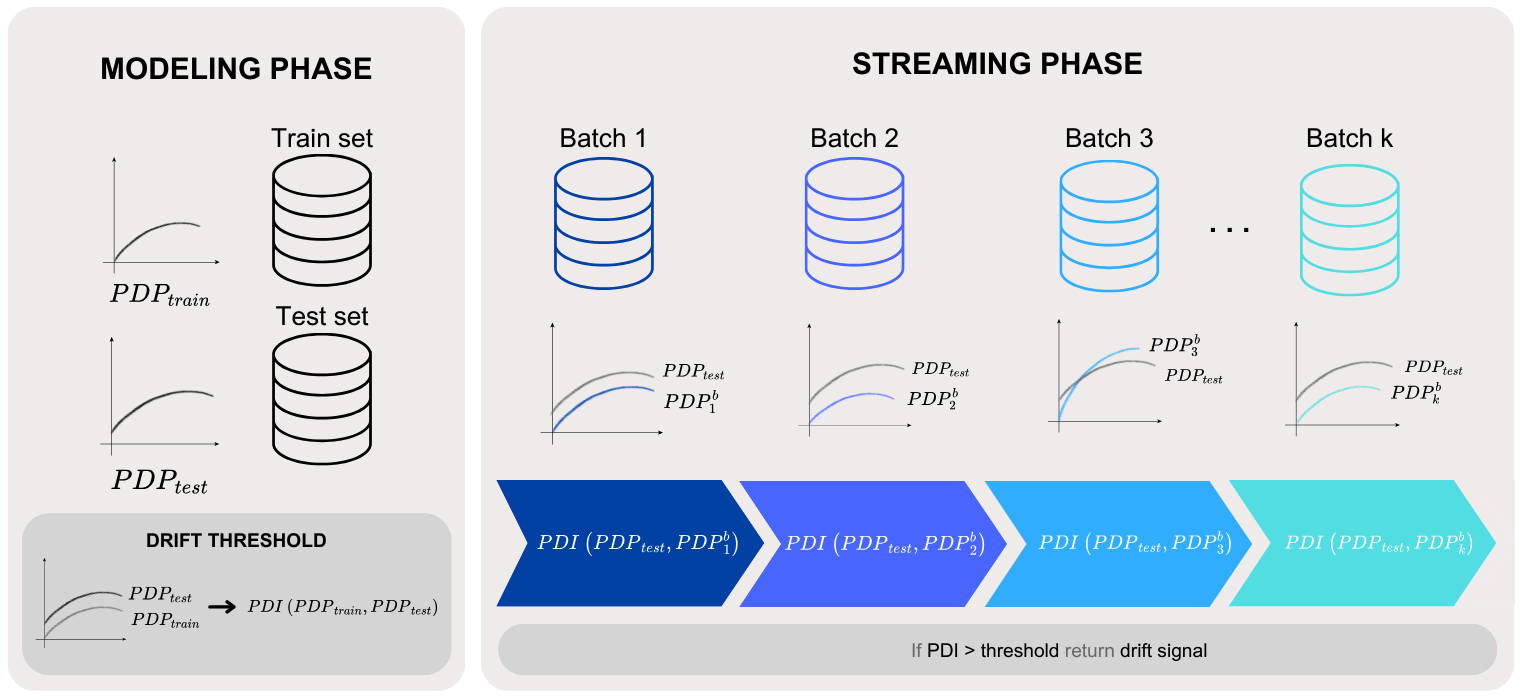
\includegraphics[width=0.8\linewidth,height=0.2\textheight]{figures/pdd_resize} 

}

\caption{The workflow of the Profile Drift Detection}\label{fig:pdd}
\end{figure}

PDD allows parameterization of three metrics: PDI, L2 and L2Der. Previous studies \citep{dar_2023, dar_2024} found PDI alone insufficient for detecting concept drift. PDD enhances detection by incorporating L2 and L2Der, with thresholds set to allow acceptable deviations.

\hypertarget{using-package}{%
\section{\texorpdfstring{Using \CRANpkg{datadriftR} package}{Using  package}}\label{using-package}}

The \CRANpkg{datadriftR} package detects concept drift in real-time data streams using various statistical methods, including DDM, EDDM, HDDM-A, HDDM-W, KSWIN, PH and PDD. These methods are based on established research and can be applied in both dynamic and static data environments.

The package is implemented using the R6 object-oriented paradigm, enhancing flexibility and encapsulation for complex data scenarios.

Below is an example of generating a data stream and applying DDM for drift detection using \CRANpkg{datadriftR}:

\begin{verbatim}
> library(datadriftR)

# Generate a sample data stream of 1000 elements with equal probabilities for 0 and 1
> set.seed(123)  # Setting a seed for reproducibility
> data_part1 <- sample(c(0, 1), size = 500, replace = TRUE, prob = c(0.7, 0.3))

# Introduce a change in data distribution
> data_part2 <- sample(c(0, 1), size = 500, replace = TRUE, prob = c(0.3, 0.7))

# Combine the two parts
> data_stream <- c(data_part1, data_part2)

# Initialize the DDM object
> ddm <- DDM$new()

# Iterate through the data stream
> for (i in seq_along(data_stream)) {
   ddm$add_element(data_stream[i])
   if (ddm$change_detected) {
     message(paste("Drift detected!", i))
   } else if (ddm$warning_detected) {
     # message(paste("Warning detected at position:", i))
   }
}

Drift detected! 560
\end{verbatim}

This example demonstrates initializing the DDM detector, processing a simulated data stream and detecting drift at position 560. The same approach applies to EDDM, HDDM-A, HDDM-W, KSWIN and PH by initializing their respective classes.

The \texttt{ProfileDifference} class calculates differences between profiles using various methods, including PDD. Below is an example:

\begin{verbatim}
> profile1 <- list(x = seq(0, 10, length.out = 100), y = sin(seq(0, 10, length.out = 100)))
> profile2 <- list(x = seq(0, 10, length.out = 100), y = cos(seq(0, 10, length.out = 100)))
> pdd <- ProfileDifference$new(method = "pdi", deriv = "gold")

> pdd$set_profiles(profile1, profile2)
> result <- pdd$calculate_difference()
> print(result$distance)
[1] 0.5154639
\end{verbatim}

This method is adaptable to various configurations, making \texttt{ProfileDifference} a flexible tool for profile comparisons in dynamic data environments.

\hypertarget{experiments}{%
\section{Experiments}\label{experiments}}

In this section, traditional methods and the PDD method are compared using synthetic and real-world datasets frequently used. The characteristics of the benchmark dataset and the design of the experiment are described.

\hypertarget{datasets}{%
\subsection{Datasets}\label{datasets}}

In the experiments, we used the generic synthetic and real-world datasets \texttt{SEA} \citep{street_and_kim_2001}, \texttt{Hyperplane} \citep{hulten_et_al_2001}, \texttt{NOAA} \citep{elwell_polikar_2011}, \texttt{Ozone} \citep{zhang_and_fan_2008}, \texttt{Elec2} \citep{harries_1999} and \texttt{Friedman} \citep{ikonomovska_et_al_2011}. The characteristics of these datasets are provided in Table\textasciitilde{}\ref{tab:dataset}.

\begin{table}[H]
    \centering
    \small
    \caption{The characteristics of the benchmark dataset}
    \label{tab:dataset}
    \begin{tabular}{lllrr}\toprule
    \textbf{Dataset}        & \textbf{Type} & \textbf{Task}     & \textbf{\#observations}   & \textbf{\#variables} \\\midrule
    \texttt{SEA}            & Synthetic     & Classification    & 50000            & 4\\
    \texttt{Hyperplane}     & Synthetic     & Classification    & 20000            & 3\\
    \texttt{NOAA}           & Real          & Classification    & 18159            & 9\\
    \texttt{Ozone}          & Real          & Classification    & 2534             & 73\\
    \texttt{Elec2}          & Real          & Classification    & 45312            & 9\\
    \texttt{Friedman}       & Synthetic     & Regression        & 20000            & 11\\\bottomrule
    \end{tabular}
\end{table}

\hypertarget{design-of-experiments}{%
\subsection{Design of experiments}\label{design-of-experiments}}

Experiments were conducted using Logistic Regression (LR), Decision Tree (DT) and Random Forest (RF). For the Friedman dataset, Linear Regression replaced LR.

For each incoming batch, its suitability for training was evaluated using PDI, L2Der and L2 calculated from PDPs. If all three exceeded their thresholds, the batch was added to the training set and the model was retrained. When PDD detected concept drift, PDP curves for train-test sets and graphs at the drift point were recorded, ensuring continuous model adaptation.

Statistical tests verified whether the response variable was correctly predicted. If drift was detected, similar incoming data was added to the training set, followed by retraining.

Tables\textasciitilde{}\ref{tab:exp_SEA}-\ref{tab:exp_Friedman} summarize the drift detection methods, batch numbers, test-train sizes, detected drifts and model performance. Large batch sizes may miss drifts, while small sizes may cause false detections, making optimal batch size selection critical.

Additional details on batch sizes (Table\textasciitilde{}\ref{tab:batch_number}), key variables (Table\textasciitilde{}\ref{tab:vip_batch}) and model accuracy (Table\textasciitilde{}\ref{tab:acc_batch}) are provided in supplemantal materials section.

\hypertarget{results}{%
\subsection{Results}\label{results}}

In this section, the results of experiments conducted on the datasets---\texttt{SEA}, \texttt{Hyperplane}, \texttt{NOAA}, \texttt{Ozone}, \texttt{Elec2} and \texttt{Friedman}---are summarized. The methods' performance is evaluated based on accuracy and the number of detected drifts (\texttt{\#drifts}).

\hypertarget{section}{%
\subsubsection{\texorpdfstring{\texttt{SEA}}{}}\label{section}}

The PDI metric was excluded due to shape similarity and L2/L2Der cutoff values were set as five times the test set values in logistic regression model in this experiment. Table\textasciitilde{}\ref{tab:exp_SEA} evaluates the performance of drift detection methods across models. PDD generally achieved high accuracy, particularly with 10 batches, where LR and RF performed competitively or better than other methods. KSWIN and EDDM also showed high accuracy but detected significantly more drifts, indicating potential over-sensitivity. HDDM-A and HDDM-W detected fewer drifts, especially with smaller batches, while maintaining accuracy comparable to PDD. PH demonstrated stable drift detection but had lower accuracy than PDD. DDM either failed to detect drifts or detected very few, suggesting lower sensitivity.

\begin{table}[H]
    \centering
    \small
    \caption{The results of experiments on the \texttt{SEA} dataset}
    \label{tab:exp_SEA}
    \begin{tabular}{llcccccc}\toprule
        && \multicolumn{6}{c}{\textbf{\#batch}}\\\cmidrule(lr){3-8}
        && \multicolumn{2}{c}{\textbf{10}}    & \multicolumn{2}{c}{\textbf{20}} & \multicolumn{2}{c}{\textbf{30}} \\\cmidrule(lr){3-8}
        \textbf{Method} & \textbf{Model} & \textbf{accuracy} & \textbf{\#drifts} & \textbf{accuracy} & \textbf{\#drifts} & \textbf{accuracy} & \textbf{\#drifts} \\\midrule
        HDDM-A & LR & 0.8306 & 1 & 0.8462 & 2 & 0.8447 & 2 \\
        & DT & 0.8318 & 2 & 0.8400 & 2 & 0.8358 & 2 \\
        & RF & 0.8264 & 1 & 0.8432 & 2 & 0.8384 & 2 \\
        \midrule
        HDDM-W & LR & 0.8279 & 3 & 0.8443 & 2 & 0.8407 & 2 \\
        & DT & 0.8248 & 3 & 0.8389 & 2 & 0.8354 & 2 \\
        & RF & 0.8257 & 3 & 0.8412 & 4 & 0.8362 & 3 \\
        \midrule
        KSWIN & LR & 0.8292 & 10 & 0.8455 & 20 & 0.8428 & 27 \\
        & DT & 0.8294 & 10 & 0.8440 & 20 & 0.8376 & 29 \\
        & RF & 0.8268 & 10 & 0.8421 & 20 & 0.8387 & 29 \\
        \midrule
        PH & LR & 0.8337 & 1 & 0.8447 & 3 & 0.8437 & 3 \\
        & DT & 0.8307 & 1 & 0.8424 & 3 & 0.8368 & 3 \\
        & RF & 0.8298 & 1 & 0.8417 & 3 & 0.8393 & 3 \\
        \midrule
        DDM & LR & 0.8284 & 0 & 0.8460 & 3 & 0.8426 & 5 \\
        & DT & 0.8267 & 0 & 0.8432 & 1 & 0.8356 & 3 \\
        & RF & 0.8267 & 0 & 0.8430 & 3 & 0.8379 & 3 \\
        \midrule
        EDDM & LR & 0.8292 & 10 & 0.8455 & 20 & 0.8381 & 12 \\
        & DT & 0.8291 & 9 & 0.8435 & 18 & 0.8340 & 8 \\
        & RF & 0.8268 & 10 & 0.8423 & 19 & 0.8390 & 13 \\
        \midrule
        PDD & LR & 0.8309 & 5 & 0.8464 & 18 & 0.8370 & 1 \\
        & DT & 0.8230 & 1 & 0.8405 & 3 & 0.8349 & 8 \\
        & RF & 0.8283 & 5 & 0.8427 & 8 & 0.8377 & 18 \\
        \midrule
    \end{tabular}
\end{table}

PDD detected drifts in a more controlled manner, reducing false positives and ensuring stable performance, especially in medium and large batch sizes. In contrast, KSWIN and EDDM detected more drifts, increasing false positives, while HDDM-A and HDDM-W detected fewer, potentially missing actual changes. PH and DDM showed moderate detection, varying by drift characteristics.

By model type, PDD maintained high accuracy in LR while detecting fewer drifts for stability. In DT and RF, it provided consistent results with fewer detections than other methods. RF showed high accuracy but KSWIN and EDDM detected more drifts, increasing operational noise.

PDD's advantages include reducing false positives, maintaining accuracy across models and batch sizes and ensuring stability, making it reliable for evolving data streams.

LR detected five drifts in the 10th batch. As shown in Figure\textasciitilde{}\ref{fig:sealogistic}, PDPs between train and test sets remained similar, indicating consistent model performance. Even after drift detection, PDPs retained their shape. PDI was 0 at drift points, confirming stable functional relationships despite distribution shifts.

\begin{figure}[H]

{\centering 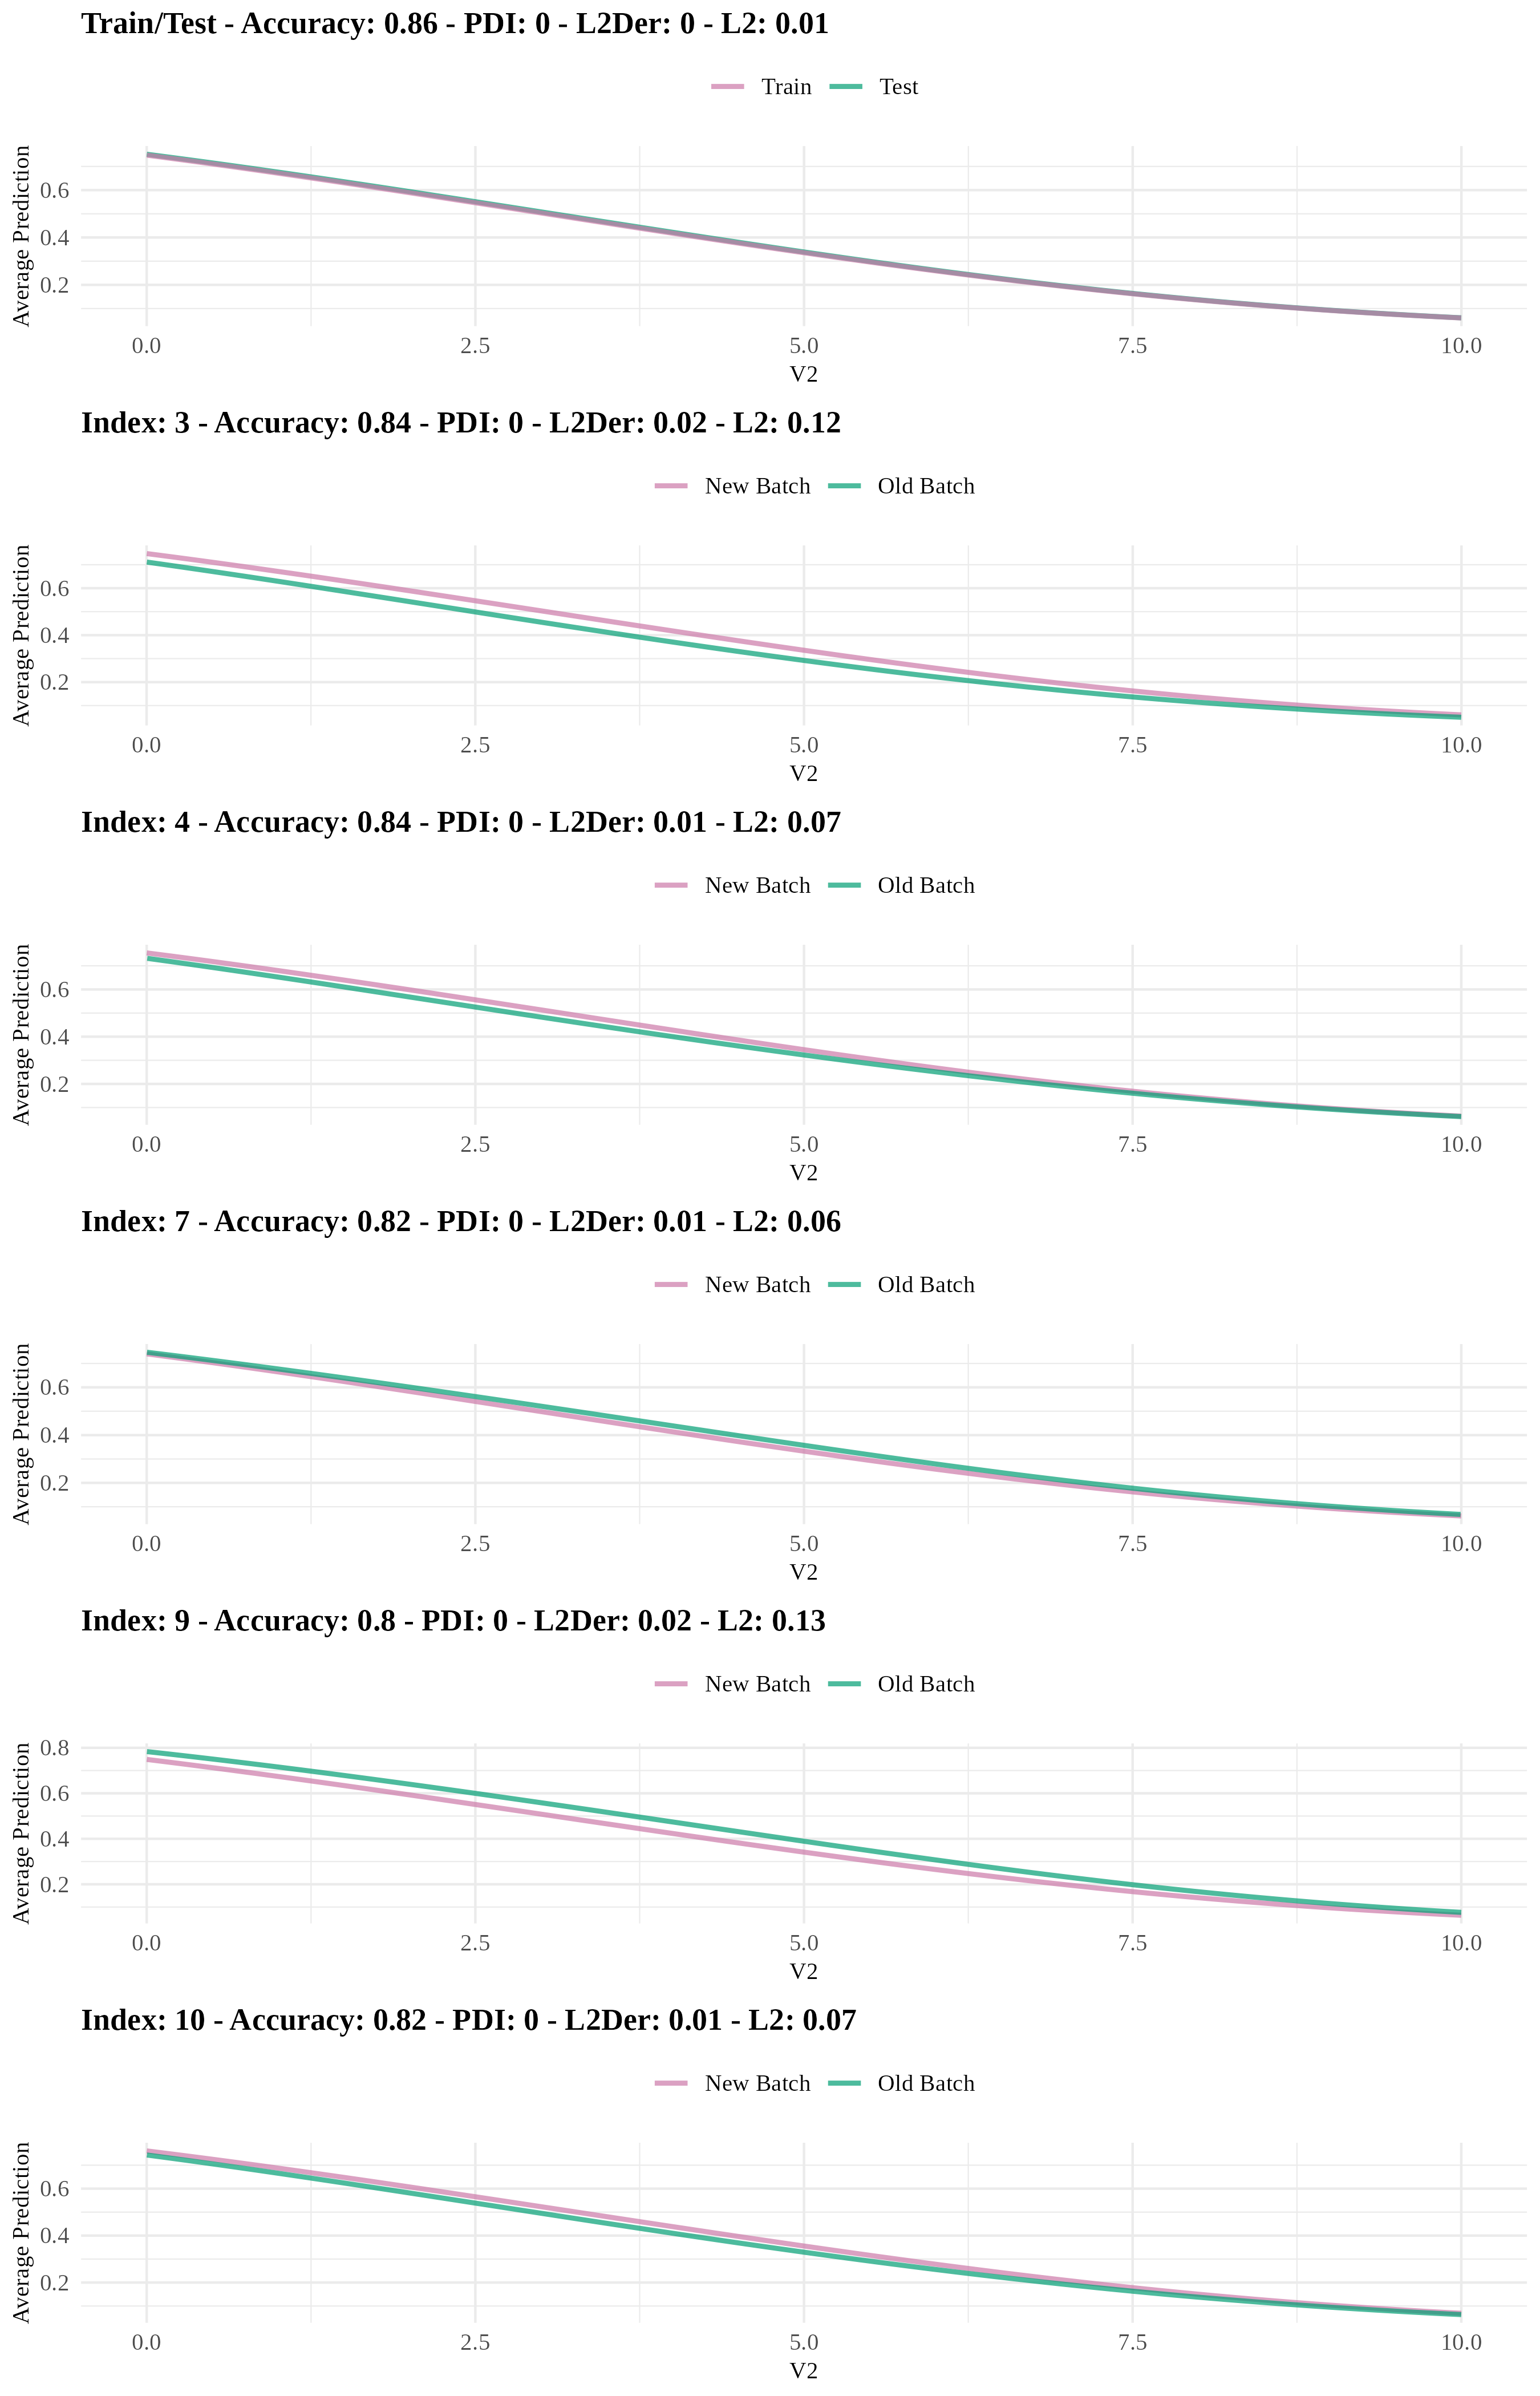
\includegraphics[width=0.95\linewidth]{figures/sea_logistic_10} 

}

\caption{PDPs of the Logistic Regression model trained on \texttt{SEA} dataset}\label{fig:sealogistic}
\end{figure}

For the DT model, a drift was detected at the 4th index. As shown in Figure\textasciitilde{}\ref{fig:seadecisiontree}, variable \texttt{V1} significantly contributed to this drift. Specifically, within the range of 0 to 5, \texttt{V1}'s influence on the response variable declined, indicating a weakened predictive power. This suggests a shift in the relationship between \texttt{V1} and the target variable, likely due to changes in data distribution. Such shifts emphasize the need to monitor variable contributions over time, as subtle alterations can signal drifts that may impact model performance.

\begin{figure}[H]

{\centering 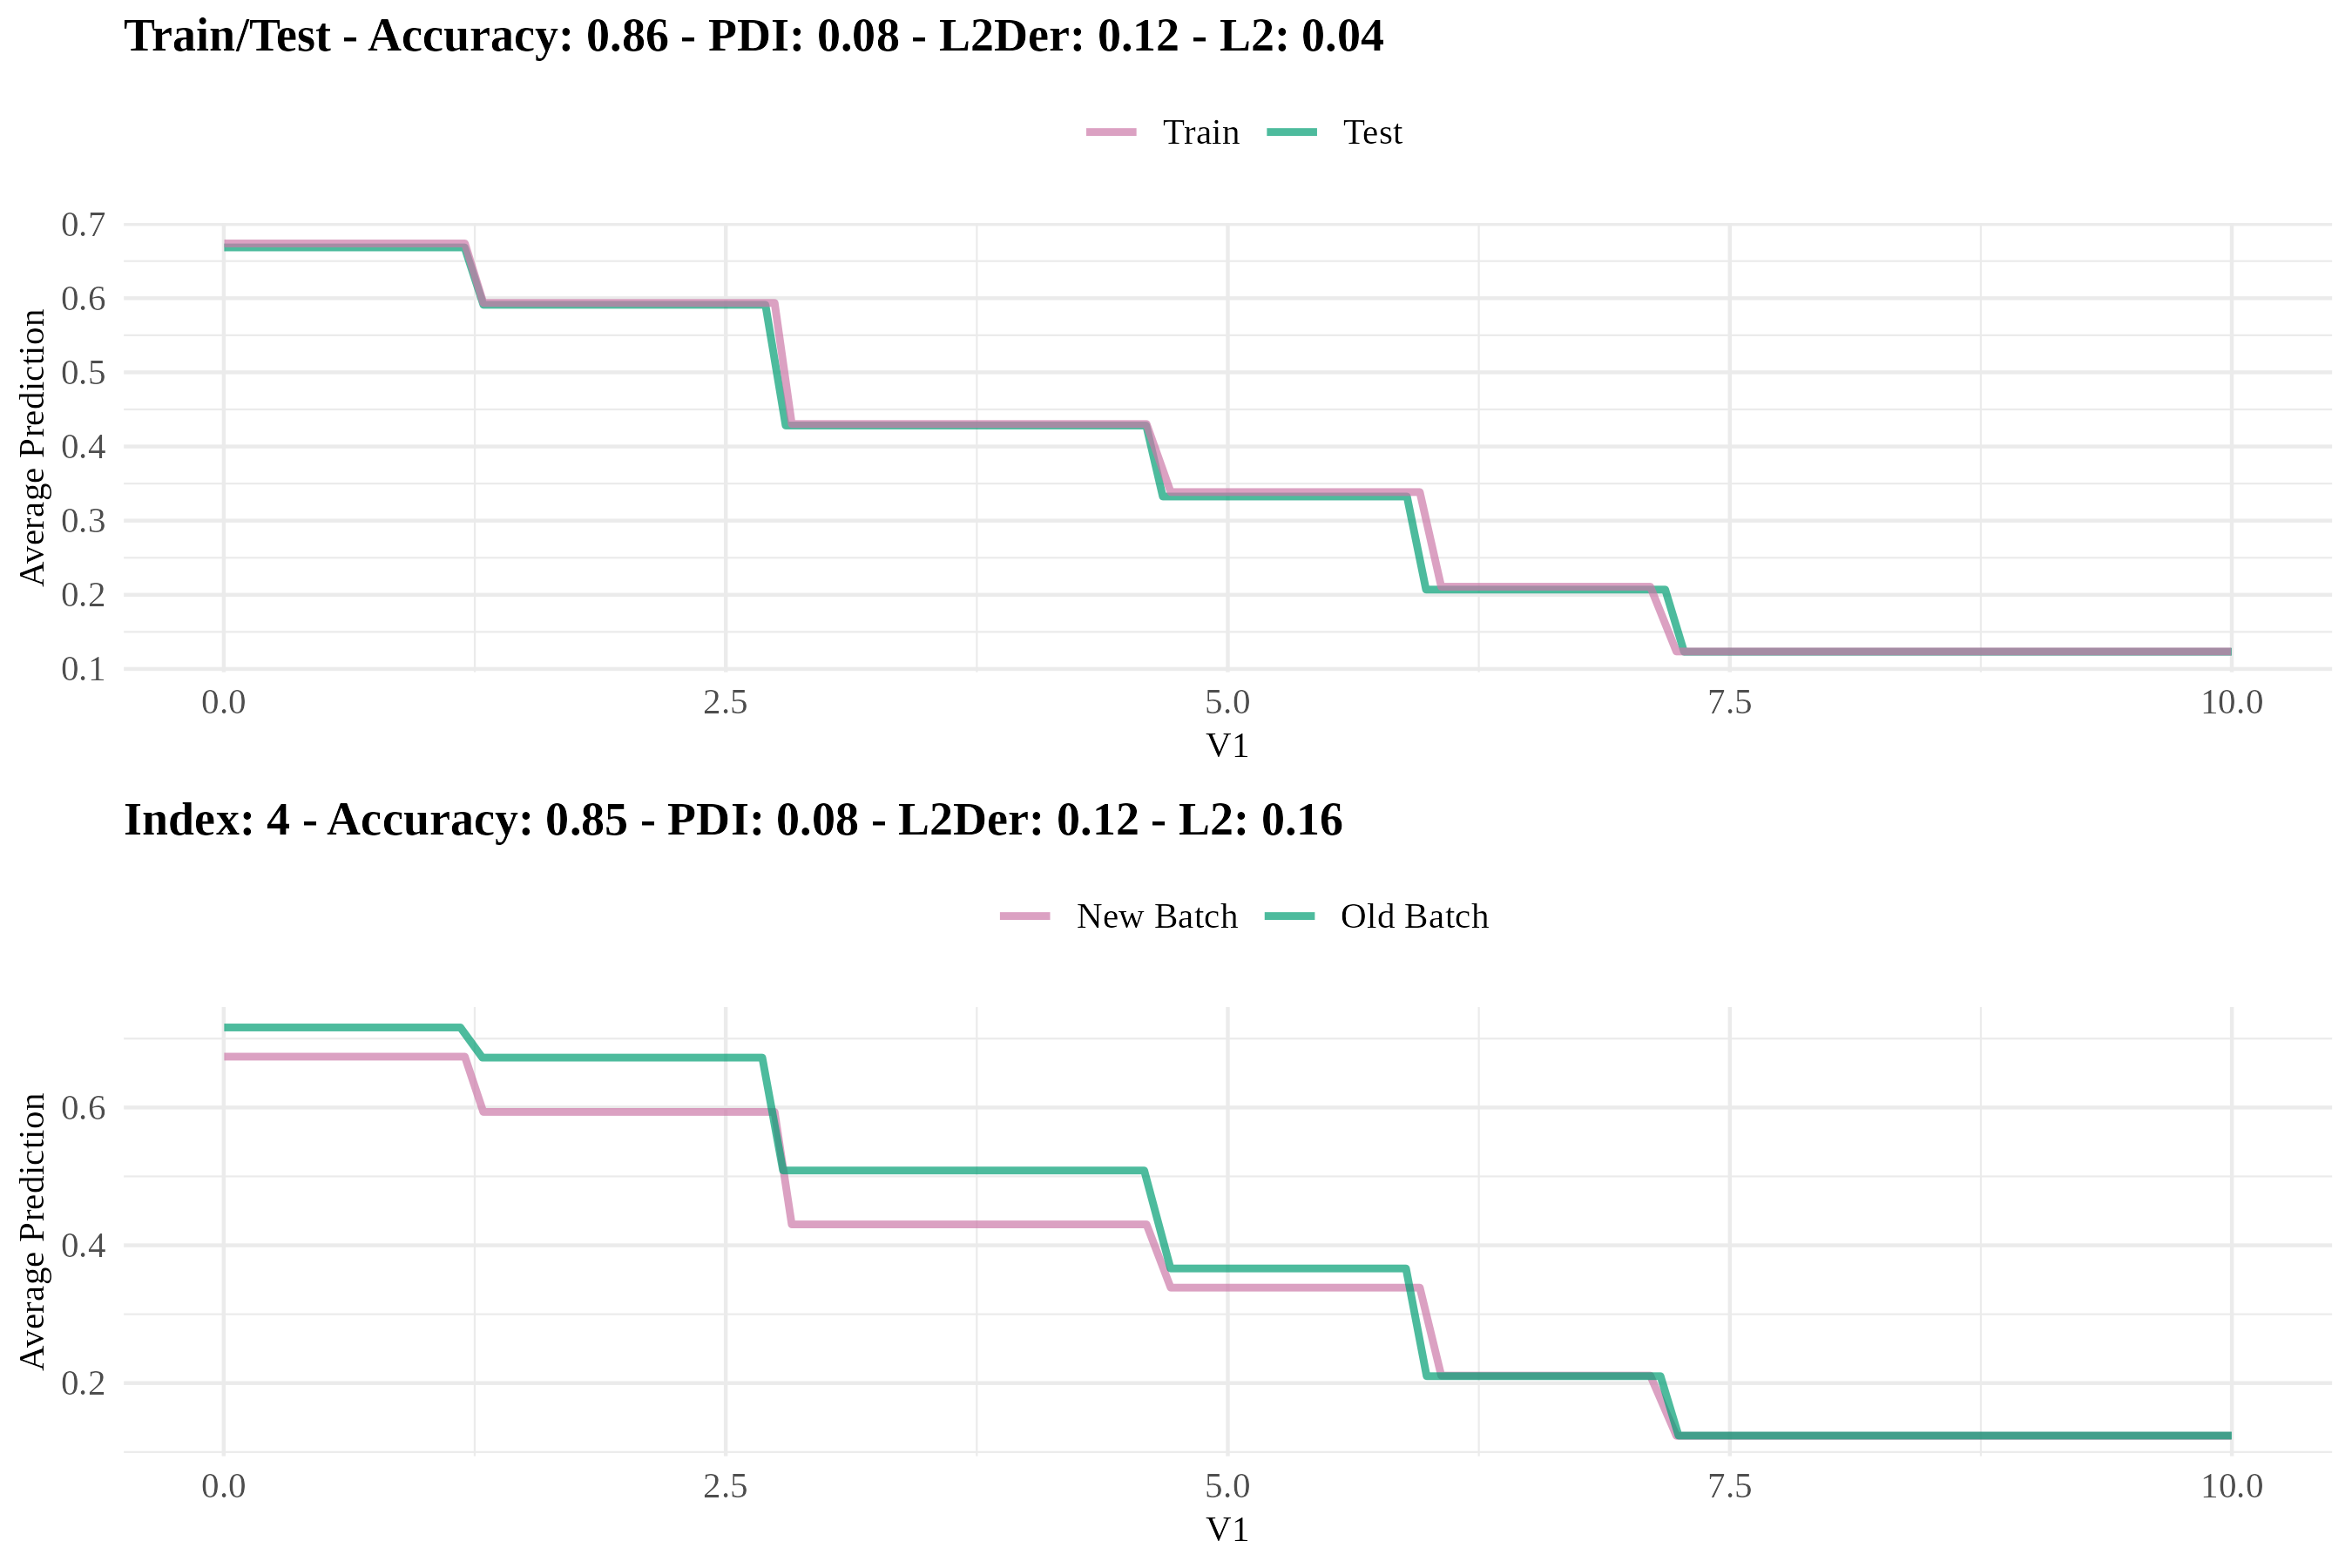
\includegraphics[width=0.95\linewidth]{figures/sea_dt_10} 

}

\caption{PDPs of the Decision Tree model trained on \texttt{SEA} dataset}\label{fig:seadecisiontree}
\end{figure}

Variable \texttt{V2} was identified as the most important feature in the RF model. Figure\textasciitilde{}\ref{fig:searandomforest} shows that \texttt{V2} played a key role at the 3rd and 10th indices. Within the range of 0 to 7.5, noticeable variations in \texttt{V2}'s behavior suggest a shift in its influence on the model's output, likely due to data distribution changes in these batches. These shifts highlight how variations in key variables can impact model performance and generalization. Monitoring important variables is crucial, as small changes can trigger drift detection and necessitate model adaptation, especially in real-time data streams.

\begin{figure}[H]

{\centering 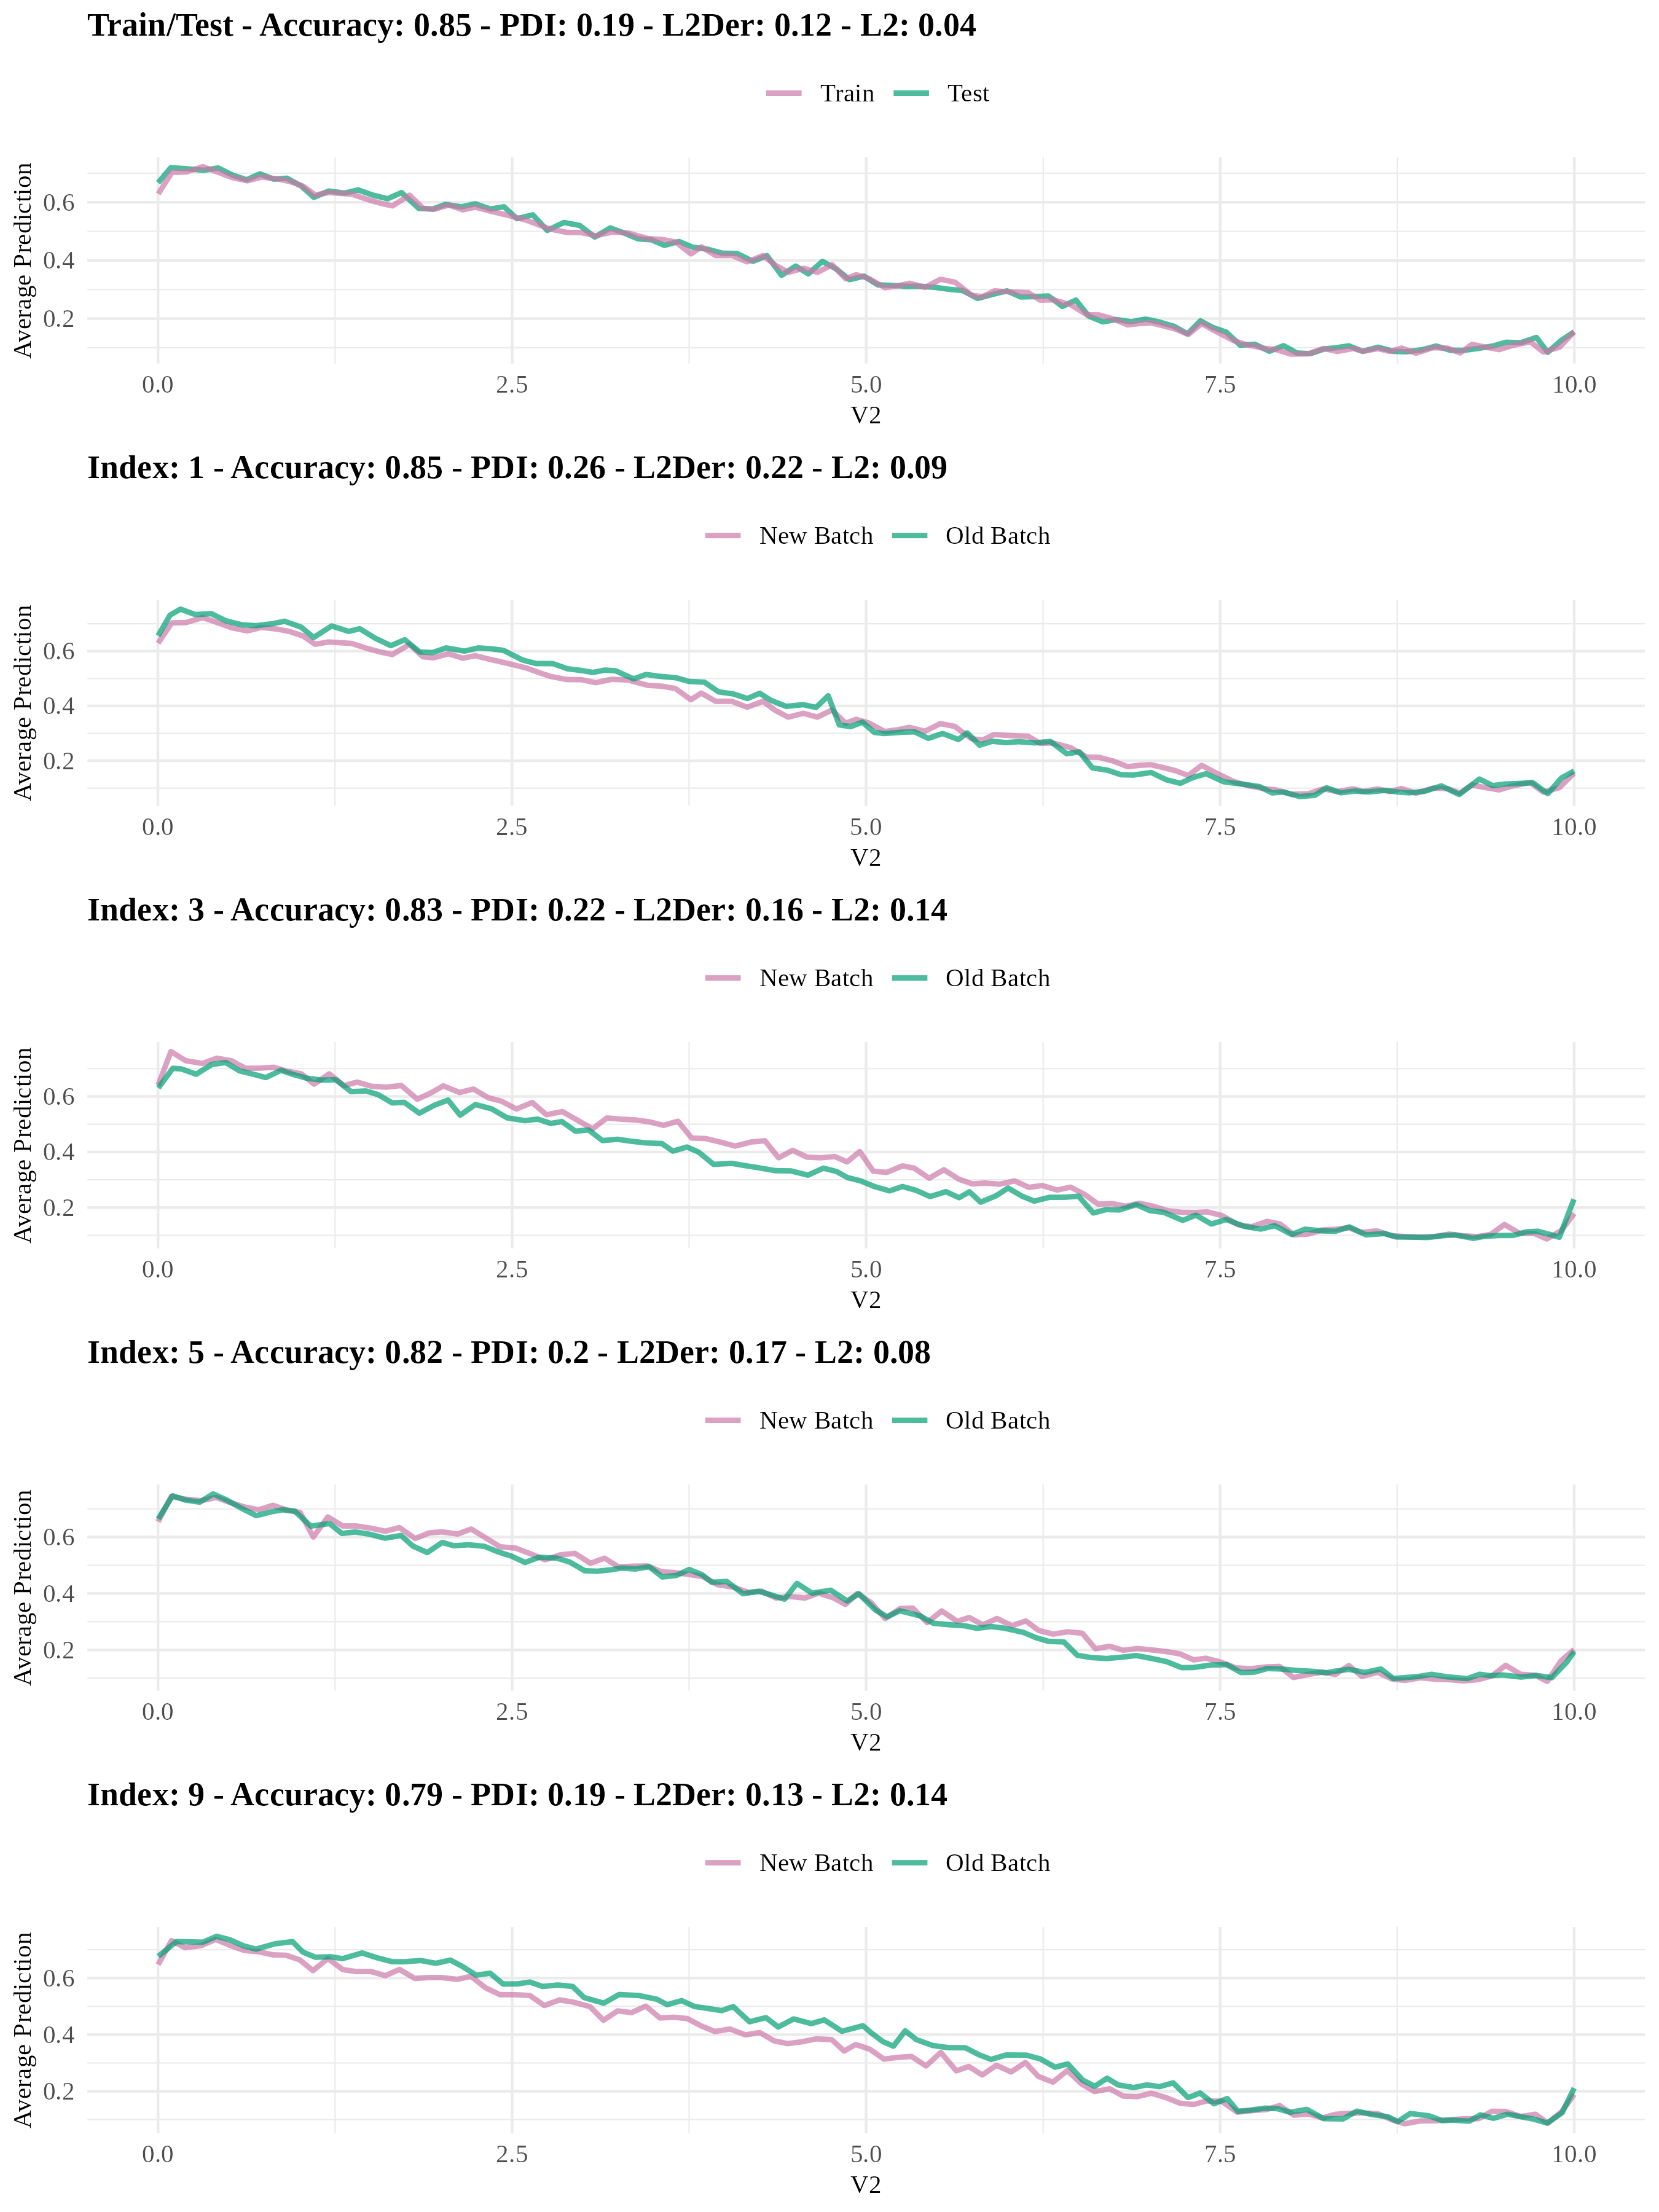
\includegraphics[width=0.95\linewidth]{figures/sea_rf_10} 

}

\caption{PDPs of the Random Forest model trained on \texttt{SEA} dataset}\label{fig:searandomforest}
\end{figure}

\hypertarget{section-1}{%
\subsubsection{\texorpdfstring{\texttt{Hyperplane}}{}}\label{section-1}}

Table\textasciitilde{}\ref{tab:exp_Hyperplane} shows that for the \texttt{Hyperplane} dataset, the PDD method achieved competitive accuracy at 10 and 20 batches in DT and RF models. The LR model reached 0.8648 accuracy with 10 batches, comparable to KSWIN and EDDM. However, as batches increased to 30, PDD's accuracy dropped significantly to 0.5219 for LR, indicating reduced performance beyond 20 batches.

\begin{table}[H]
    \centering
    \small
    \caption{The results of experiments on the \texttt{Hyperplane} dataset}
    \label{tab:exp_Hyperplane}
    \begin{tabular}{llcccccc}\toprule
        && \multicolumn{6}{c}{\textbf{\#batch}}\\\cmidrule(lr){3-8}
        && \multicolumn{2}{c}{\textbf{10}}    & \multicolumn{2}{c}{\textbf{20}} & \multicolumn{2}{c}{\textbf{30}} \\\cmidrule(lr){3-8}
        \textbf{Method} & \textbf{Model} & \textbf{accuracy} & \textbf{\#drifts} & \textbf{accuracy} & \textbf{\#drifts} & \textbf{accuracy} & \textbf{\#drifts} \\\midrule
        HDDM-A & LR & 0.8662 & 1 & 0.8204 & 2 & 0.7568 & 3 \\
        & DT & 0.8398 & 0 & 0.7670 & 3 & 0.6921 & 3 \\
        & RF & 0.7834 & 0 & 0.6809 & 1 & 0.6267 & 1 \\
        \midrule
        HDDM-W & LR & 0.8377 & 1 & 0.8456 & 3 & 0.8152 & 4 \\
        & DT & 0.8398 & 0 & 0.7752 & 2 & 0.7316 & 4 \\
        & RF & 0.7794 & 2 & 0.7615 & 3 & 0.7536 & 6 \\
        \midrule
        KSWIN & LR & 0.8639 & 9 & 0.8458 & 13 & 0.8285 & 18 \\
        & DT & 0.8520 & 9 & 0.8429 & 17 & 0.8162 & 19 \\
        & RF & 0.8219 & 10 & 0.8144 & 17 & 0.7948 & 22 \\
        \midrule
        PH & LR & 0.8648 & 0 & 0.8187 & 1 & 0.7455 & 2 \\
        & DT & 0.8398 & 0 & 0.7014 & 1 & 0.6929 & 1 \\
        & RF & 0.7834 & 0 & 0.7033 & 1 & 0.6267 & 1 \\
        \midrule
        DDM & LR & 0.8648 & 0 & 0.8071 & 1 & 0.7455 & 2 \\
        & DT & 0.8398 & 0 & 0.7014 & 1 & 0.7283 & 3 \\
        & RF & 0.7834 & 0 & 0.7290 & 3 & 0.6267 & 1 \\
        \midrule
        EDDM & LR & 0.8648 & 0 & 0.8485 & 13 & 0.8348 & 5 \\
        & DT & 0.8496 & 10 & 0.8562 & 15 & 0.8379 & 11 \\
        & RF & 0.7834 & 0 & 0.8072 & 16 & 0.7957 & 24 \\
        \midrule
        PDD & LR & 0.8648 & 0 & 0.6469 & 1 & 0.5219 & 0 \\
        & DT & 0.8435 & 1 & 0.8326 & 15 & 0.4924 & 1 \\
        & RF & 0.7831 & 1 & 0.7322 & 4 & 0.5099 & 0 \\
        \midrule
    \end{tabular}
\end{table}

An analysis of train-test accuracies suggests overfitting, particularly in RF. For LR, training accuracy was \(0.7320\), while test accuracy dropped from \(0.6165\) (10 batches) to \(0.5113\) (30 batches). Similar trends in DT and RF indicate overfitting, likely impacting PDD's drift detection.

PDD identified fewer drifts under overfitting, whereas KSWIN and EDDM detected up to 22. This suggests PDD reduces false positives but may miss actual drifts in overfitting scenarios.

KSWIN and EDDM detected more drifts, increasing sensitivity but also false positives. HDDM-A and HDDM-W detected fewer drifts, balancing sensitivity and stability. PH showed moderate detection, while DDM performed inconsistently, especially in RF.

Overall, PDD balanced accuracy and drift detection in the \texttt{Hyperplane} dataset, especially at 20 batches. However, its performance declined outside this range due to overfitting. While PDD minimizes false positives, its sensitivity to actual drifts may be limited when model generalization is affected.

\hypertarget{section-2}{%
\subsubsection{\texorpdfstring{\texttt{NOAA}}{}}\label{section-2}}

The results for the \texttt{NOAA} dataset in Table\textasciitilde{}\ref{tab:exp_NOAA} show that PDD performed effectively mainly at 20 batches. For LR, accuracy increased from \(0.7649\) (10 batches) to \(0.7708\) (30 batches) but drift detections were minimal, with 0 drifts at 10 and 30 batches and only 2 at 20 batches.

\begin{table}[H]
    \centering
    \small
    \caption{The results of experiments on the \texttt{NOAA} dataset}
    \label{tab:exp_NOAA}
    \begin{tabular}{llcccccc}\toprule
        && \multicolumn{6}{c}{\textbf{\#batch}}\\\cmidrule(lr){3-8}
        && \multicolumn{2}{c}{\textbf{10}}    & \multicolumn{2}{c}{\textbf{20}} & \multicolumn{2}{c}{\textbf{30}} \\\cmidrule(lr){3-8}
        \textbf{Method} & \textbf{Model} & \textbf{accuracy} & \textbf{\#drifts} & \textbf{accuracy} & \textbf{\#drifts} & \textbf{accuracy} & \textbf{\#drifts} \\\midrule
        HDDM-A & LR & 0.7736 & 5 & 0.7696 & 7 & 0.7777 & 3 \\
        & DT & 0.7293 & 8 & 0.7435 & 9 & 0.7440 & 8 \\
        & RF & 0.7790 & 0 & 0.7783 & 4 & 0.7780 & 2 \\
        \midrule
        HDDM-W & LR & 0.7736 & 7 & 0.7712 & 12 & 0.7799 & 12 \\
        & DT & 0.7385 & 10 & 0.7345 & 16 & 0.7385 & 23 \\
        & RF & 0.7883 & 4 & 0.7835 & 10 & 0.7826 & 9 \\
        \midrule
        KSWIN & LR & 0.7755 & 10 & 0.7755 & 20 & 0.7788 & 27 \\
        & DT & 0.7385 & 10 & 0.7334 & 20 & 0.7437 & 29 \\
        & RF & 0.7916 & 10 & 0.7916 & 19 & 0.7945 & 29 \\
        \midrule
        PH & LR & 0.7707 & 3 & 0.7680 & 3 & 0.7792 & 3 \\
        & DT & 0.7402 & 2 & 0.7387 & 2 & 0.7276 & 2 \\
        & RF & 0.7869 & 3 & 0.7798 & 3 & 0.7772 & 3 \\
        \midrule
        DDM & LR & 0.7716 & 4 & 0.7746 & 10 & 0.7715 & 10 \\
        & DT & 0.7422 & 3 & 0.7334 & 20 & 0.7398 & 21 \\
        & RF & 0.7818 & 1 & 0.7914 & 20 & 0.7831 & 8 \\
        \midrule
        EDDM & LR & 0.7755 & 10 & 0.7755 & 20 & 0.7780 & 30 \\
        & DT & 0.7385 & 10 & 0.7334 & 20 & 0.7406 & 30 \\
        & RF & 0.7916 & 10 & 0.7914 & 20 & 0.7940 & 30 \\
        \midrule
        PDD & LR & 0.7649 & 0 & 0.7694 & 2 & 0.7708 & 0 \\
        & DT & 0.7264 & 2 & 0.7403 & 0 & 0.7352 & 3 \\
        & RF & 0.7881 & 5 & 0.7676 & 0 & 0.7913 & 22 \\
        \midrule
    \end{tabular}
\end{table}

Overfitting is a primary issue in the RF model, with train accuracy reaching \(0.9998\) while test accuracy ranges from \(0.7723\) to \(0.8338\). In contrast, LR and DT show smaller train-test gaps, indicating minimal overfitting.

PDD detected fewer drifts in overfitting scenarios, especially in RF, identifying 22 drifts at 30 batches compared to 29 and 30 detected by KSWIN and EDDM. While reducing false positives, PDD risks missing actual drifts in overfitting conditions.

Other methods varied: KSWIN and EDDM detected more drifts but increased false positives, HDDM-A and HDDM-W balanced sensitivity and stability, PH detected fewer drifts and DDM showed moderate sensitivity.

Overall, PDD showed limited effectiveness in the \texttt{NOAA} dataset. KSWIN and EDDM provided more consistent drift detection but at the cost of higher false positives.

\hypertarget{section-3}{%
\subsubsection{\texorpdfstring{\texttt{Ozone}}{}}\label{section-3}}

The results for the \texttt{Ozone} dataset, shown in Table\textasciitilde{}\ref{tab:exp_Ozone}, highlight varied performances across drift detection methods, models and batch sizes. The PDD method achieved moderate accuracy, with \(0.9353\) at 10 batches, \(0.8984\) at 20 batches and \(0.8724\) at 30 batches in the LR model. While PDD maintained a consistent number of detected drifts for LR, its performance slightly declined as batch size increased.

\begin{table}[H]
    \centering
    \small
    \caption{The results of experiments on the \texttt{Ozone} dataset}
    \label{tab:exp_Ozone}
    \begin{tabular}{llcccccc}\toprule
        && \multicolumn{6}{c}{\textbf{\#batch}}\\\cmidrule(lr){3-8}
        && \multicolumn{2}{c}{\textbf{10}}    & \multicolumn{2}{c}{\textbf{20}} & \multicolumn{2}{c}{\textbf{30}} \\\cmidrule(lr){3-8}
        \textbf{Method} & \textbf{Model} & \textbf{accuracy} & \textbf{\#drifts} & \textbf{accuracy} & \textbf{\#drifts} & \textbf{accuracy} & \textbf{\#drifts} \\\midrule
        HDDM-A & LR & 0.9294 & 0 & 0.8942 & 2 & 0.8116 & 0 \\
        & DT & 0.9487 & 0 & 0.9101 & 1 & 0.9036 & 2 \\
        & RF & 0.9508 & 0 & 0.9427 & 1 & 0.9374 & 0 \\
        \midrule
        HDDM-W & LR & 0.9294 & 0 & 0.8907 & 1 & 0.8526 & 1 \\
        & DT & 0.9487 & 0 & 0.9101 & 1 & 0.9122 & 2 \\
        & RF & 0.9508 & 0 & 0.9427 & 1 & 0.9401 & 1 \\
        \midrule
        KSWIN & LR & 0.9396 & 3 & 0.9164 & 2 & 0.9144 & 5 \\
        & DT & 0.9444 & 3 & 0.9242 & 4 & 0.9099 & 5 \\
        & RF & 0.9529 & 1 & 0.9383 & 4 & 0.9437 & 3 \\
        \midrule
        PH & LR & 0.9294 & 0 & 0.8502 & 0 & 0.8116 & 0 \\
        & DT & 0.9487 & 0 & 0.8911 & 0 & 0.8725 & 0 \\
        & RF & 0.9508 & 0 & 0.9422 & 0 & 0.9374 & 0 \\
        \midrule
        DDM & LR & 0.9406 & 4 & 0.9155 & 6 & 0.8706 & 2 \\
        & DT & 0.9358 & 7 & 0.9301 & 6 & 0.9329 & 4 \\
        & RF & 0.9513 & 2 & 0.9427 & 2 & 0.9437 & 3 \\
        \midrule
        EDDM & LR & 0.9396 & 2 & 0.9183 & 4 & 0.8842 & 6 \\
        & DT & 0.9412 & 2 & 0.9164 & 4 & 0.9185 & 5 \\
        & RF & 0.9524 & 2 & 0.9441 & 3 & 0.9437 & 3 \\
        \midrule
        PDD & LR & 0.9353 & 1 & 0.8984 & 2 & 0.8724 & 2 \\
        & DT & 0.9487 & 0 & 0.8915 & 1 & 0.9140 & 10 \\
        & RF & 0.9508 & 5 & 0.9422 & 0 & 0.9455 & 12 \\
        \midrule
    \end{tabular}
\end{table}

In the DT model, PDD detected one drift at 20 batches, rising to ten at 30. For RF, it identified five drifts at 10 batches, none at 20 and twelve at 30, suggesting sensitivity depends on model complexity.

The target distribution (2374 to 160) impacts drift detection. At 30 batches, PDD detected more drifts than other methods, achieving the highest accuracy (0.9455). Unlike response-based methods, PDD provides deeper insights via PDP comparisons.

Other methods varied in performance: DDM, KSWIN and EDDM detected more drifts but increased false positives, while HDDM-A and HDDM-W balanced sensitivity and stability with fewer detections.

Key variables shifted across models and batch sizes, highlighting the need for adaptive selection. \texttt{V26} was crucial in LR at 10 batches, shifting to \texttt{V52} at 20/30; DT's key variable changed from \texttt{V31} to \texttt{V36} and RF's from \texttt{V56} to \texttt{V61}.

In summary, PDD maintained accuracy while detecting fewer drifts, particularly in overfitting-prone RF models. It reduced false positives but may miss key drifts, whereas KSWIN and EDDM offered more consistent detection at the cost of increased false alarms. Adaptive variable selection and a combination of methods may enhance drift detection.

\hypertarget{section-4}{%
\subsubsection{\texorpdfstring{\texttt{Elec2}}{}}\label{section-4}}

The results for the \texttt{Elec2} dataset highlight distinct performance patterns across drift detection methods, models and batch sizes. The PDD method demonstrated a balanced approach in accuracy and drift detection.

For the Logistic Regression (LR) model, PDD achieved accuracies of \(0.6740\), \(0.7349\) and \(0.7402\) for \(10\), \(20\) and \(30\) batches, respectively. In the DT model, accuracies remained consistent at \(0.7253\), \(0.7392\) and \(0.7449\), while in the RF model, accuracies were \(0.7093\), \(0.7311\) and \(0.7393\) across the same batch sizes.

\begin{table}[H]
    \centering
    \small
    \caption{The results of experiments on the \texttt{Elec2} dataset}
    \label{tab:exp_Elec2}
    \begin{tabular}{llcccccc}\toprule
        && \multicolumn{6}{c}{\textbf{\#batch}}\\\cmidrule(lr){3-8}
        && \multicolumn{2}{c}{\textbf{10}}    & \multicolumn{2}{c}{\textbf{20}} & \multicolumn{2}{c}{\textbf{30}} \\\cmidrule(lr){3-8}
        \textbf{Method} & \textbf{Model} & \textbf{accuracy} & \textbf{\#drifts} & \textbf{accuracy} & \textbf{\#drifts} & \textbf{accuracy} & \textbf{\#drifts} \\\midrule
        HDDM-A & LR & 0.6983 & 10 & 0.6836 & 20 & 0.7099 & 30 \\
        & DT & 0.7255 & 10 & 0.7409 & 20 & 0.7450 & 30 \\
        & RF & 0.7029 & 10 & 0.7243 & 20 & 0.7374 & 30 \\
        \midrule
        HDDM-W & LR & 0.6983 & 10 & 0.6836 & 20 & 0.7099 & 30 \\
        & DT & 0.7255 & 10 & 0.7409 & 20 & 0.7450 & 30 \\
        & RF & 0.7029 & 10 & 0.7243 & 20 & 0.7374 & 30 \\
        \midrule
        KSWIN & LR & 0.6983 & 10 & 0.6836 & 20 & 0.7099 & 30 \\
        & DT & 0.7255 & 10 & 0.7409 & 20 & 0.7450 & 30 \\
        & RF & 0.7029 & 10 & 0.7243 & 20 & 0.7374 & 30 \\
        \midrule
        PH & LR & 0.6983 & 10 & 0.7342 & 13 & 0.7390 & 16 \\
        & DT & 0.7215 & 9 & 0.7417 & 15 & 0.7502 & 16 \\
        & RF & 0.6992 & 8 & 0.7103 & 11 & 0.7368 & 16 \\
        \midrule
        DDM & LR & 0.6983 & 10 & 0.6836 & 20 & 0.7099 & 30 \\
        & DT & 0.7255 & 10 & 0.7409 & 20 & 0.7450 & 30 \\
        & RF & 0.7029 & 10 & 0.7250 & 16 & 0.7253 & 17 \\
        \midrule
        EDDM & LR & 0.6983 & 10 & 0.6836 & 20 & 0.7099 & 30 \\
        & DT & 0.7255 & 10 & 0.7409 & 20 & 0.7450 & 30 \\
        & RF & 0.7029 & 10 & 0.7243 & 20 & 0.7374 & 30 \\
        \midrule
        PDD & LR & 0.6740 & 8 & 0.7349 & 4 & 0.7402 & 12 \\
        & DT & 0.7253 & 1 & 0.7392 & 1 & 0.7429 & 5 \\
        & RF & 0.7093 & 3 & 0.7311 & 0 & 0.7449 & 3 \\
        \midrule
    \end{tabular}
\end{table}

When comparing PDD to other drift detection methods, it exhibits a moderate number of drift detections. In the LR model, PDD detected \(8\), \(4\) and \(12\) drifts across \(10\), \(20\) and \(30\) batches, respectively. In DT, drift detections were minimal, with \(1\) drift at \(10\) and \(20\) batches, increasing to \(5\) at \(30\) batches. The RF model showed \(3\), \(0\) and \(3\) drifts for the same batch sizes. This controlled detection suggests that PDD effectively identifies significant changes while minimizing false positives.

Other methods, such as HDDM-A, HDDM-W, KSWIN and EDDM, detected drifts equal to the batch size across all models. PH exhibited an increasing trend, detecting up to \(16\) drifts in all models at \(30\) batches. DDM showed a rising number of drifts, particularly in RF, indicating high sensitivity.

Accuracy-wise, most methods maintained strong performance across models and batch sizes. The LR model consistently achieved accuracies above \(0.68\), while DT and RF models surpassed \(0.70\)-\(0.74\). High base test and train accuracies indicate overall robust model performance.

A key finding in the \texttt{Elec2} dataset is that \texttt{nswprice} was the most influential variable across all models and batch sizes, emphasizing its critical role in predictive performance. With \(30\) batches, RF achieved its highest accuracy when updated three times using PDD. Other methods detected more drifts but did not match this accuracy.

In summary, PDD demonstrated balanced performance on \texttt{Elec2}, maintaining accuracy while controlling drift detections. Its conservative approach reduces false positives, making it advantageous in scenarios requiring stable drift detection. The identification of \texttt{nswprice} as the key variable underscores the need for focused variable analysis in drift detection and model evaluation. Overall, PDD provides a reliable balance between accuracy and drift sensitivity.

\begin{figure}[H]

{\centering 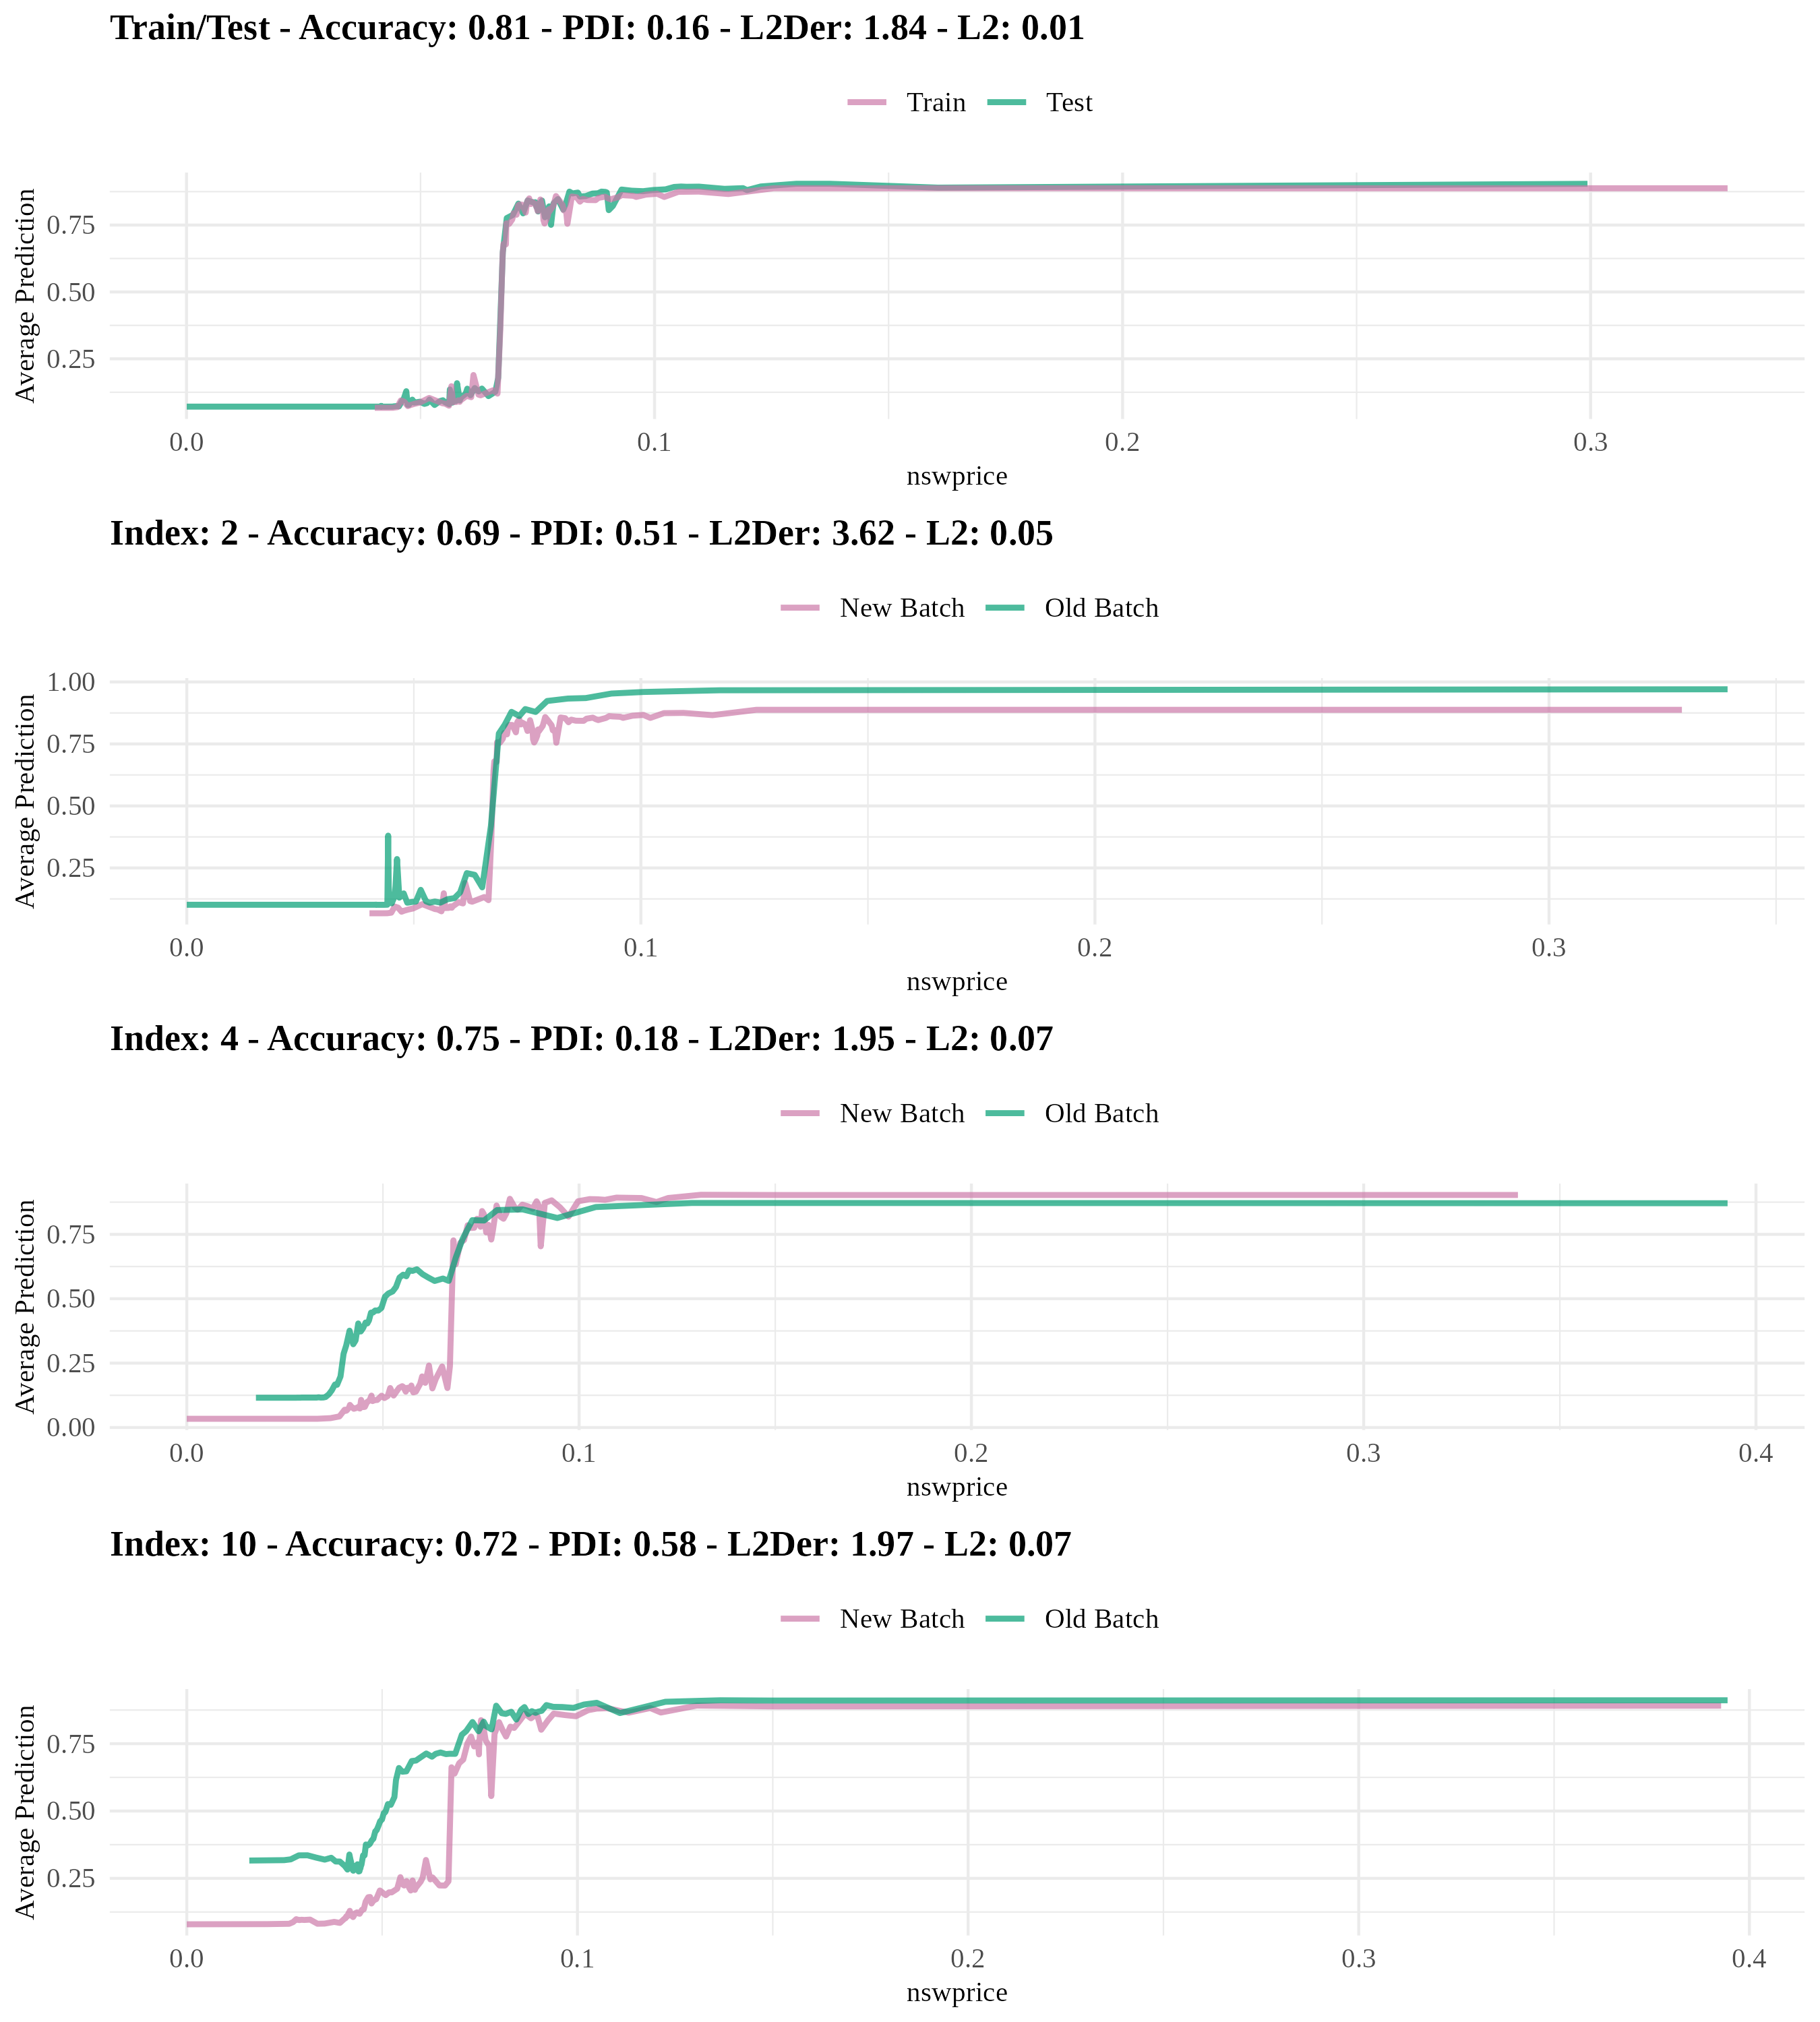
\includegraphics[width=0.8\linewidth]{figures/rf_elec_10} 

}

\caption{PDPs of the Random Forest model trained on \texttt{Elec2} dataset}\label{fig:rfelec10}
\end{figure}

For the RF model applied to the \texttt{Elec2} dataset, drift was detected in the 10th batch. As shown in Figure\textasciitilde{}\ref{fig:rfelec10}, the \texttt{nswprice} variable, the most important feature, exhibits noticeable changes between \(0\) and \(0.1\). In this range, its contribution to the model's predictions shifts, triggering drift detection by PDD. These variations indicate how \texttt{nswprice} influences the model differently in the 10th batch, potentially affecting its performance.

\hypertarget{section-5}{%
\subsubsection{\texorpdfstring{\texttt{Friedman}}{}}\label{section-5}}

The results for the \texttt{Friedman} dataset in Table\textasciitilde{}\ref{tab:exp_Friedman}, a regression task, show distinct performance patterns across drift detection methods, models and batch sizes. The PDD method demonstrated a balanced approach in both metric values and drift detection. The PDI metric was excluded due to shape similarity in this experiment.

\begin{table}[H]
    \centering
    \small
    \caption{The results of experiments on the \texttt{Friedman} dataset}
    \label{tab:exp_Friedman}
    \begin{tabular}{llcccccc}\toprule
        && \multicolumn{6}{c}{\textbf{\#batch}}\\\cmidrule(lr){3-8}
        && \multicolumn{2}{c}{\textbf{10}}    & \multicolumn{2}{c}{\textbf{20}} & \multicolumn{2}{c}{\textbf{30}} \\\cmidrule(lr){3-8}
        \textbf{Method} & \textbf{Model} & \textbf{accuracy} & \textbf{\#drifts} & \textbf{accuracy} & \textbf{\#drifts} & \textbf{accuracy} & \textbf{\#drifts} \\\midrule
        KSWIN & LR & 2.8029 & 10 & 2.8007 & 19 & 2.7906 & 30 \\
        & DT & 3.2977 & 10 & 3.2765 & 19 & 3.2921 & 23 \\
        & RF & 1.9021 & 10 & 1.9280 & 19 & 1.9320 & 26 \\
        \midrule
        PH & LR & 2.8023 & 5 & 2.7974 & 10 & 2.7812 & 9 \\
        & DT & 3.3254 & 9 & 3.2813 & 16 & 3.2752 & 16 \\
        & RF & 1.9613 & 2 & 2.0566 & 4 & 2.0115 & 7 \\
        \midrule
        PDD & LR & 2.8041 & 3 & 2.8073 & 2 & 2.7998 & 1 \\
        & DT & 3.3014 & 3 & 3.2936 & 2 & 3.2670 & 2 \\
        & RF & 1.9887 & 7 & 1.8811 & 4 & 1.9355 & 11 \\
        \midrule
    \end{tabular}
\end{table}

KSWIN detected the highest number of drifts across all models and batch sizes. In LR, it identified \(10\), \(19\) and \(30\) drifts, with RMSE slightly decreasing from \(2.8029\) to \(2.7906\). Similarly, DT and RF models showed \(10\), \(19\) and \(23\) drifts and \(10\), \(20\) and \(24\) drifts, respectively, with minor RMSE improvements. While highly sensitive, KSWIN's frequent detections increase false positive risks.

PH showed moderate sensitivity, detecting fewer drifts than KSWIN but more than PDD. In LR, PH detected \(5\), \(10\) and \(9\) drifts, improving RMSE from \(2.8023\) to \(2.7812\). DT detected \(9\), \(16\) and \(16\) drifts, while RF detected \(2\), \(4\) and \(7\), maintaining stable metrics. PH balances sensitivity and stability, making it suitable for controlled drift detection.

Across all methods, \texttt{variable\_4} consistently emerged as the key feature, emphasizing its importance in model performance and drift detection.

In summary, PDD controlled drift detections while maintaining reasonable metrics in the \texttt{Friedman} dataset. It reduced false positives but was less sensitive than KSWIN, which detected more drifts but increased false alarms. PH offered a balanced approach, while the stability of \texttt{variable\_4} highlights the need for adaptive variable selection in drift detection.

\hypertarget{conclusions}{%
\section{Conclusions}\label{conclusions}}

In this paper, we conducted six experiments on real and synthetic datasets to compare PDD with common drift detection methods (HDDM-A, HDDM-W, KSWIN, PH, DDM, EDDM). We analyzed model accuracy, detected drifts and variable contributions during drift events.

PDD evaluates three metrics---PDI, L2 and L2Der---between PDP curves. Thresholds are set using train-test PDPs and new batch metrics are compared against them. Experiments also tested alternative conditions, such as exceeding thresholds in at least two metrics. Statistical tests and PDD were compared across batch sizes in terms of drift detection and model performance.

Beyond detecting drift, PDD provides insights into model-variable relationships. Unlike traditional methods that rely on response prediction, PDD detects changes even at high accuracy levels, allowing updates when data relationships shift without affecting standard metrics.

PDD balanced drift detection and accuracy, avoiding excessive false positives. It performed stably on \texttt{SEA} and \texttt{Elec2}, while in \texttt{Hyperplane}, \texttt{NOAA} and \texttt{Ozone}, overfitting impacted its drift detection. In \texttt{Friedman}, PDD effectively minimized false positives while maintaining accuracy.

Comparatively, KSWIN and EDDM were highly sensitive, detecting more drifts but increasing false positives. PH and DDM offered moderate detection, balancing stability and sensitivity.

Key variables consistently influenced drift detection, such as \texttt{V2} in \texttt{SEA}, \texttt{nswprice} in \texttt{Elec2} and \texttt{variable\_4} in \texttt{Friedman}, underscoring the need for monitoring influential attributes in dynamic data environments.

\hypertarget{discussion}{%
\section{Discussion}\label{discussion}}

Beyond detecting drift, PDD provides insights into predictive churn, helping explain model changes after retraining \citep{daniels_2024}. Unlike statistical methods, PDD clarifies model-data relationships, aiding users in understanding drift causes. It can also contribute to data privacy challenges, such as removing learned relationships from models \citep{bourtoule_2021}.

PDD has limitations, including computational cost and infeasibility for multi-class classification. Derivative calculations are difficult for categorical variables and relying on the most important variable may overlook drifts from other features, requiring broader analysis and increasing computational demands. Sparse vectors can also exaggerate PDI metric variations.

PDD is suited for binary classification and regression but adapting it for multi-class tasks is costly.

In conclusion, PDD balances drift detection with model interpretability. It detects fewer but more consistent drifts while maintaining accuracy, offering deeper insights into how explanatory variables influence concept drift.

\hypertarget{further-research}{%
\section{Further research}\label{further-research}}

To reduce PDD's computational cost, the \textit{compress then explain} technique \citep{hubert_2024} can be integrated, compressing large datasets before applying explainable methods. When model training is costly, PDD can be used as is. If PDP generation is more expensive than model training, PDD can track changes in response-explanatory variable relationships. Additionally, PDD aids in predictive churn and data privacy by explaining changes after ML model retraining.

\hypertarget{acknowledgment}{%
\subsection{Acknowledgment}\label{acknowledgment}}

The work on this paper is financially supported by the Scientific and Technological Research Council
of Turkiye under the 2210C National MSc Scholarship Program in the Priority Fields in Science and
Technology grant no. 1649B022303919 and Eskisehir Technical University Scientific Research Projects
Commission under grant no. 22LÖT175.

\hypertarget{supplemantal-materials}{%
\subsection{Supplemantal materials}\label{supplemantal-materials}}

The materials for reproducing the experiments performed and the dataset are
accessible in the following repository: \url{https://github.com/ugurdar/datadrift\_RJournal}

\begin{table}[H]
    \centering
    \small
    \caption{The number of observations in the batches}
    \label{tab:batch_number}
    \begin{tabular}{lrrrrrr}\toprule
                & \multicolumn{6}{c}{\textbf{\#batch}}\\\cmidrule(lr){2-7}
                & \multicolumn{2}{c}{\textbf{10}} & \multicolumn{2}{c}{\textbf{20}} & \multicolumn{2}{c}{\textbf{30}} \\\cmidrule(lr){2-7}
        \textbf{Dataset} & \textbf{train} & \textbf{test} & \textbf{train} & \textbf{test} & \textbf{train} & \textbf{test} \\\midrule
        \texttt{SEA} & 13332 & 3334 & 8000 & 2000 & 5713 & 1429 \\
        \texttt{Hyperplane} & 5332 & 1334 & 3200 & 800 & 2285 & 572 \\
        \texttt{NOAA} & 4842 & 1211 & 2904 & 727 & 2075 & 519 \\
        \texttt{Ozone} & 675 & 169 & 404 & 102 & 289 & 73 \\
        \texttt{Elec2} & 12083 & 3021 & 7249 & 1813 & 5178 & 1295 \\
        \texttt{Friedman} & 5332 & 1334 & 3200 & 800 & 2285 & 572 \\
        \bottomrule
    \end{tabular}
\end{table}

\begin{table}[H]
    \centering
    \small
    \caption{The most important variables in the batches}
    \label{tab:vip_batch}
    \begin{tabular}{llccc}\toprule
                            &       & \multicolumn{3}{c}{\textbf{\#batch}}\\\cmidrule(lr){3-5}
        \textbf{Dataset}    & \textbf{Model} & \textbf{10}                    & \textbf{20}                    & \textbf{30} \\\midrule
        \texttt{SEA} & LR & \texttt{V2} & \texttt{V2} & \texttt{V2} \\
                            & DT & \texttt{V1} & \texttt{V1} & \texttt{V1} \\
                            & RF & \texttt{V2} & \texttt{V2} & \texttt{V2} \\
        \midrule
        \texttt{Hyperplane} & LR & \texttt{feature\_1} & \texttt{feature\_1} & \texttt{feature\_1} \\
                            & DT & \texttt{feature\_1} & \texttt{feature\_1} & \texttt{feature\_2} \\
                            & RF & \texttt{feature\_1} & \texttt{feature\_1} & \texttt{feature\_1} \\
        \midrule
        \texttt{NOAA} & LR & \texttt{attribute1} & \texttt{attribute4} & \texttt{attribute1} \\
                            & DT & \texttt{attribute2} & \texttt{attribute2} & \texttt{attribute2} \\
                            & RF & \texttt{attribute2} & \texttt{attribute4} & \texttt{attribute2} \\
        \midrule
        \texttt{Ozone} & LR & \texttt{V26} & \texttt{V52} & \texttt{V52} \\
                            & DT & \texttt{V31} & \texttt{V36} & \texttt{V36} \\
                            & RF & \texttt{V56} & \texttt{V61} & \texttt{V61} \\
        \midrule
        \texttt{Elec2} & LR & \texttt{nswprice} & \texttt{nswprice} & \texttt{nswprice} \\
                            & DT & \texttt{nswprice} & \texttt{nswprice} & \texttt{nswprice} \\
                            & RF & \texttt{nswprice} & \texttt{nswprice} & \texttt{nswprice} \\
        \midrule
        \texttt{Friedman} & LR & \texttt{feature\_4} & \texttt{feature\_4} & \texttt{feature\_4} \\
                            & DT & \texttt{feature\_4} & \texttt{feature\_4} & \texttt{feature\_4} \\
                            & RF & \texttt{feature\_4} & \texttt{feature\_4} & \texttt{feature\_4} \\
        \midrule
    \end{tabular}
\end{table}

\begin{table}[H]
    \centering
    \small
    \caption{The accuracies of the models in the batches}
    \label{tab:acc_batch}
    \begin{tabular}{llcccccc}\toprule
    & & \multicolumn{6}{c}{\textbf{\#batch}}\\
    \cmidrule(lr){3-8}
    & & \multicolumn{2}{c}{\textbf{10}} & \multicolumn{2}{c}{\textbf{20}} & \multicolumn{2}{c}{\textbf{30}} \\
    \cmidrule(lr){3-8}
    \textbf{Dataset} & \textbf{Model} & \textbf{test} & \textbf{train} & \textbf{test} & \textbf{train} & \textbf{test} & \textbf{train} \\
    \midrule
    \texttt{SEA} & LR & 0.8579 & 0.8966 & 0.8946 & 0.9032 & 0.9007 & 0.9057 \\
                          & DT & 0.8576 & 0.8801 & 0.8696 & 0.8850 & 0.8797 & 0.8850 \\
                          & RF & 0.8537 & 0.9991 & 0.8896 & 0.9989 & 0.9007 & 0.9991 \\
    \midrule
    \texttt{Hyperplane} & LR & 0.6165 & 0.7320 & 0.6717 & 0.7122 & 0.5113 & 0.7580 \\
                          & DT & 0.7079 & 0.7406 & 0.7266 & 0.7094 & 0.4276 & 0.7575 \\
                          & RF & 0.6524 & 0.9992 & 0.6692 & 0.9984 & 0.4799 & 0.9978 \\
    \midrule
    \texttt{NOAA} & LR & 0.7748 & 0.7999 & 0.8118 & 0.8041 & 0.8173 & 0.8014 \\
                          & DT & 0.7500 & 0.7881 & 0.7734 & 0.7996 & 0.7808 & 0.7990 \\
                          & RF & 0.7723 & 0.9996 & 0.8338 & 0.9997 & 0.8154 & 0.9995 \\
    \midrule
    \texttt{Ozone} & LR & 0.9647 & 0.9526 & 0.8155 & 1.0000 & 0.9054 & 1.0000 \\
                          & DT & 0.9882 & 0.9511 & 0.8544 & 0.9554 & 0.9730 & 0.9308 \\
                          & RF & 0.9941 & 1.0000 & 0.9806 & 1.0000 & 1.0000 & 1.0000 \\
    \midrule
    \texttt{Elec2} & LR & 0.8154 & 0.8200 & 0.8043 & 0.8081 & 0.8156 & 0.8188 \\
                          & DT & 0.7955 & 0.8264 & 0.8649 & 0.8238 & 0.8025 & 0.8316 \\
                          & RF & 0.8107 & 0.8424 & 0.8142 & 0.8367 & 0.8040 & 0.8418 \\
    \midrule
    \texttt{Friedman} & LR & 2.6432 & 2.5926 & 2.5591 & 2.5579 & 2.5958 & 2.5463 \\
                          & DT & 3.0254 & 2.9843 & 3.1574 & 2.9204 & 3.0400 & 2.9744 \\
                          & RF & 1.6395 & 0.7275 & 1.7751 & 0.7659 & 1.7454 & 0.8102 \\
    \midrule
    \end{tabular}
\end{table}

\hypertarget{references}{%
\section{References}\label{references}}

\bibliography{RJreferences.bib}

\address{%
Ugur Dar\\
Eskisehir Technical University\\%
Department of Statistics, Eskisehir, Turkey\\
%
%
\textit{ORCiD: \href{https://orcid.org/0009-0005-8076-2199}{0009-0005-8076-2199}}\\%
\href{mailto:ugurdarr@gmail.com}{\nolinkurl{ugurdarr@gmail.com}}%
}

\address{%
Mustafa Cavus\\
Eskisehir Technical University\\%
Department of Statistics, Eskisehir, Turkey\\
%
%
\textit{ORCiD: \href{https://orcid.org/0000-0002-6172-5449}{0000-0002-6172-5449}}\\%
\href{mailto:mustafacavus@eskisehir.edu.tr}{\nolinkurl{mustafacavus@eskisehir.edu.tr}}%
}
